% lecture12_ro.tex -- GENERATED by build_L12.py from L12_numbers.json; do not edit by hand.
\documentclass[10pt,aspectratio=169,t]{beamer}
% =============================================================================
% nn_preamble.tex -- shared Beamer preamble of Neural Networks and Deep Learning (NN)
% Used by every lecture: lectures/Lk/lecturek.tex does
%   \documentclass[10pt,aspectratio=169,t]{beamer}
%   % =============================================================================
% nn_preamble.tex -- shared Beamer preamble of Neural Networks and Deep Learning (NN)
% Used by every lecture: lectures/Lk/lecturek.tex does
%   \documentclass[10pt,aspectratio=169,t]{beamer}
%   % =============================================================================
% nn_preamble.tex -- shared Beamer preamble of Neural Networks and Deep Learning (NN)
% Used by every lecture: lectures/Lk/lecturek.tex does
%   \documentclass[10pt,aspectratio=169,t]{beamer}
%   \input{../common/nn_preamble}
%   \nnlecture{k}{Lecture title}
% Logos live in lectures/common/logos/, charts in lectures/Lk/charts/.
% Do NOT add \hfuzz / \vfuzz / \hbadness here: overfull boxes must be fixed, not hidden.
% =============================================================================

\usetheme{default}
\setbeamersize{text margin left=7mm, text margin right=7mm}

% ---------------------------------------------------------------- packages
\usepackage[utf8]{inputenc}
\usepackage[T1]{fontenc}
\usepackage{lmodern}
\usepackage{amsmath, amssymb}
\usepackage{mathtools}
\usepackage{bm}
\usepackage{tikz}
\usetikzlibrary{arrows.meta, positioning, calc, shapes.misc}
\usepackage{booktabs}
\usepackage{array}
\usepackage{graphicx}
\usepackage{colortbl}
\usepackage{xcolor}
\usepackage{multicol}
\hypersetup{colorlinks=true, linkcolor=MainBlue, urlcolor=MainBlue, citecolor=MainBlue}
\graphicspath{{../common/logos/}}   % charts are included with their language folder: charts/en/, charts/ro/

% ---------------------------------------------------------------- colours
\definecolor{MainBlue}{RGB}{26, 58, 110}
\definecolor{IDAred}{RGB}{205, 0, 0}
\definecolor{DarkGray}{RGB}{51, 51, 51}
\definecolor{FooterGray}{RGB}{100, 100, 100}
\definecolor{BlockGray}{RGB}{236, 238, 242}
\definecolor{KeynoteGray}{RGB}{218, 218, 218}
\definecolor{Crimson}{RGB}{190, 40, 50}
\definecolor{Forest}{RGB}{30, 110, 50}
\definecolor{Bitter}{RGB}{214, 150, 20}
% chart palette (same hex values and order as lectures/common/nn_plot.py SERIES)
\definecolor{Ser1}{HTML}{2A78D6}
\definecolor{Ser2}{HTML}{EB6834}
\definecolor{Ser3}{HTML}{1BAF7A}
\definecolor{Ser4}{HTML}{EDA100}
\definecolor{Ser5}{HTML}{E87BA4}
\definecolor{Ser6}{HTML}{008300}
\definecolor{Ser7}{HTML}{6250D6}
\definecolor{Ser8}{HTML}{E34948}

\setbeamertemplate{background}{%
  \begin{tikzpicture}[remember picture, overlay]
    \shade[shading=axis, shading angle=315, top color=white, bottom color=KeynoteGray]
      (current page.south west) rectangle (current page.north east);
  \end{tikzpicture}}
\setbeamercolor{background canvas}{bg=}
\setbeamercolor{structure}{fg=MainBlue}
\setbeamercolor{normal text}{fg=DarkGray}
\setbeamercolor{title}{fg=IDAred}
\setbeamercolor{frametitle}{fg=IDAred, bg=}
\setbeamercolor{block title}{bg=MainBlue, fg=white}
\setbeamercolor{block body}{bg=BlockGray, fg=DarkGray}
\setbeamercolor{block title alerted}{bg=Crimson, fg=white}
\setbeamercolor{block body alerted}{bg=Crimson!7, fg=DarkGray}
\setbeamercolor{block title example}{bg=Forest, fg=white}
\setbeamercolor{block body example}{bg=Forest!7, fg=DarkGray}
\setbeamercolor{item}{fg=MainBlue}
\setbeamerfont{frametitle}{size=\large, series=\bfseries}
\setbeamerfont{block title}{size=\small, series=\bfseries}
\setbeamertemplate{blocks}[rounded][shadow=false]
\setbeamertemplate{itemize item}{\color{MainBlue}$\boxdot$}
\setbeamertemplate{itemize subitem}{\color{MainBlue}\scriptsize$\blacktriangleright$}
% compact two-level lists: level 1 = main point, level 2 = details (no text outside bullets)
\setbeamerfont{itemize/enumerate subbody}{size=\footnotesize}
\setlength{\leftmargini}{1.1em}
\setlength{\leftmarginii}{1.1em}
\setbeamertemplate{itemize/enumerate body begin}{\setlength{\topsep}{0pt}\setlength{\partopsep}{0pt}\setlength{\parskip}{0pt}}
\setbeamertemplate{itemize/enumerate subbody begin}{\setlength{\topsep}{0pt}\setlength{\partopsep}{0pt}\setlength{\itemsep}{0pt}\vspace{-0.4ex}}

\setbeamertemplate{enumerate item}{\color{MainBlue}\insertenumlabel.}
\setlength{\leftmargini}{1.3em}
\setlength{\leftmarginii}{1.2em}
\setbeamertemplate{navigation symbols}{}
\setbeamertemplate{section in toc}{\color{MainBlue}$\blacktriangleright$~\inserttocsection}
\setbeamertemplate{caption}{\raggedright\insertcaption\par}
% frame subtitle = precise citation line under the claim title (Weron style)
\setbeamerfont{framesubtitle}{size=\footnotesize}
\setbeamercolor{framesubtitle}{fg=FooterGray}
% outline that reappears at every section with the current section highlighted
\setbeamertemplate{section in toc shaded}[default][35]
\setbeamertemplate{subsection in toc shaded}[default][35]
\setbeamertemplate{subsection in toc}{\leavevmode\leftskip=2.2em\color{DarkGray}\small\inserttocsubsection\par}
\AtBeginSection[]{{\begin{frame}{\txtoutline}\vspace{2mm}\small
  \tableofcontents[currentsection,hideothersubsections]\end{frame}}}

% ---------------------------------------------------------------- head and foot
\setbeamertemplate{headline}{%
  \vskip10pt%
  \hbox to \paperwidth{\hskip0.5cm%
    {\small\color{FooterGray}\renewcommand{\hyperlink}[2]{##2}\insertsectionhead}%
    \hfill\textcolor{FooterGray}{\small\insertframenumber}\hskip0.5cm}%
  \vskip4pt{\color{FooterGray}\hrule height 0.4pt}}
% footer as in the other courses (MFM, SFM): course name on the left, small sparkline on the right
\setbeamertemplate{footline}{%
  {\color{FooterGray}\hrule height 0.4pt}\vskip4pt%
  \hbox to \paperwidth{\hskip0.5cm%
    \textcolor{FooterGray}{\small\txtcourse}%
    \hfill\raisebox{-0.1em}{\begin{tikzpicture}[x=0.08em, y=0.08em, line width=0.4pt]
      \draw[FooterGray] (0,3) -- (1,4) -- (2,3.5) -- (3,5) -- (4,4) -- (5,6) -- (6,5.5) -- (7,4) -- (8,5) -- (9,7) -- (10,6) -- (11,5) -- (12,6.5) -- (13,8) -- (14,7) -- (15,6) -- (16,7.5) -- (17,9) -- (18,8) -- (19,7) -- (20,8.5) -- (21,10) -- (22,9) -- (23,8) -- (24,9.5);
    \end{tikzpicture}}\hskip0.5cm}%
  \vskip6pt}

% ---------------------------------------------------------------- title page
\defbeamertemplate*{title page}{nn}[1][]{%
  \vspace{0.15cm}
  \begin{center}
    \href{https://www.ase.ro}{
\includegraphics[height=0.9cm]{ase_logo.png}}\hspace{0.3cm}%
    \href{https://ipe.ro/new}{
\includegraphics[height=0.9cm]{acad_logo.png}}\hspace{0.3cm}%
    \href{https://theida.net}{
\includegraphics[height=0.9cm]{ida_logo.png}}\hspace{0.3cm}%
    \href{https://blockchain-research-center.com}{
\includegraphics[height=0.9cm]{brc_logo.png}}\hspace{0.3cm}%
    \href{https://www.ai4efin.ase.ro}{
\includegraphics[height=0.9cm]{ai4efin_logo.png}}\hspace{0.3cm}%
    \href{https://www.digital-finance-msca.com}{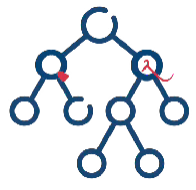
\includegraphics[height=0.9cm]{msca_logo.png}}%
  \end{center}
  \vspace{0.45cm}
  \begin{center}
    \begin{minipage}{0.1\textwidth}\centering
      \href{https://quantlet.com}{
\includegraphics[height=0.9cm]{ql_logo.png}}\end{minipage}%
    \begin{minipage}{0.78\textwidth}\centering
      {\Large\bfseries\usebeamercolor[fg]{title}\inserttitle}\par\vspace{0.25cm}
      {\large\usebeamercolor[fg]{title}\insertsubtitle}\end{minipage}%
    \begin{minipage}{0.1\textwidth}\centering
      \href{https://quantinar.com}{
\includegraphics[height=0.9cm]{qr_logo.png}}\end{minipage}
  \end{center}
  \vfill
  \hspace{0.4cm}{\bfseries\insertauthor}\par\vspace{0.12cm}
  \hspace{0.4cm}\begin{minipage}[t]{0.92\textwidth}\raggedright\footnotesize\insertinstitute\end{minipage}
  \par\vspace{0.4cm}}

% ---------------------------------------------------------------- lecture metadata
\newcommand{\nnshort}{}
\newcommand{\nnnb}{notebooks}
\newcommand{\nnrepo}{https://github.com/danpele/NEURAL_BIZ/tree/main}
% language-dependent labels (English default; \nnromanian switches to Romanian, call it before \nnlecture)
\newcommand{\txtcourse}{Neural Networks and Deep Learning}
\newcommand{\txtlecture}{Lecture}
\newcommand{\txtoutline}{Outline}
\newcommand{\txtintuition}{In one sentence:}
\newcommand{\txtjob}{In practice:}
\newcommand{\txttry}{Experiment yourself:}
\newcommand{\txtwhere}{where}
\newcommand{\txtsim}{SIMULATED DATA (teaching illustration)}
\newcommand{\txtnbsuffix}{}
\newcommand{\txtinstitute}{Bucharest University of Economic Studies (ASE), Department of Statistics and Econometrics\\
    Romanian Academy, Institute for Economic Forecasting (IPE)\\
    IDA Institute Digital Assets \textbullet\ AI4EFin \textbullet\ MSCA Digital Finance}
\newcommand{\nnromanian}{%
  \renewcommand{\txtcourse}{Rețele neuronale și deep learning}%
  \renewcommand{\txtlecture}{Cursul}%
  \renewcommand{\txtoutline}{Cuprins}%
  \renewcommand{\txtintuition}{Pe scurt:}%
  \renewcommand{\txtjob}{În practică:}%
  \renewcommand{\txttry}{Exercițiu practic:}%
  \renewcommand{\txtwhere}{unde}%
  \renewcommand{\txtsim}{DATE SIMULATE (doar pentru ilustrare)}%
  \renewcommand{\txtnbsuffix}{\string_ro}%
  \renewcommand{\txtinstitute}{Academia de Studii Economice din București (ASE), Departamentul de Statistică și Econometrie\\
    Academia Română, Institutul de Prognoză Economică (IPE)\\
    IDA Institute Digital Assets \textbullet\ AI4EFin \textbullet\ MSCA Digital Finance}}
\newcommand{\nnlecture}[2]{%
  \renewcommand{\nnshort}{\txtlecture\ #1}%
  \renewcommand{\nnnb}{notebooks/L#1\string_notebook\txtnbsuffix.ipynb}%
  \title[NN]{\txtcourse}%
  \subtitle{\txtlecture\ #1: #2}%
  \author{Prof.\ dr.\ Daniel Traian PELE}%
  \institute{\txtinstitute}%
  \date{}}

% ---------------------------------------------------------------- teaching blocks (one message per frame)
% \intuition{one plain sentence}  ->  formula with every symbol defined  ->  real-data example  ->  \manager{one line}
\newcommand{\intuition}[1]{\begin{itemize}\item {\color{MainBlue}\textbf{\txtintuition}}~#1\end{itemize}\vspace{0.6mm}}
\newcommand{\manager}[1]{\colorbox{Forest!10}{\parbox{\dimexpr\linewidth-2\fboxsep\relax}{\footnotesize
  \begin{itemize}\setlength{\itemsep}{0pt}\item \textbf{\color{Forest}\txtjob}~#1\end{itemize}}}}
% Experiment yourself: pointer to the matching notebook section
\newcommand{\tryit}[1]{{\scriptsize\href{\nnrepo/\nnnb}{%
  \raisebox{-0.15em}{
\includegraphics[height=0.85em]{ql_logo.png}}\,\textbf{\txttry}~\color{MainBlue}#1}}}
% bottom row: manager line (left) + experiment pointer (right), pinned to the bottom of the frame
\newcommand{\bottomrow}[2]{\par\vfill\noindent\begin{minipage}[b]{0.72\linewidth}#1\end{minipage}\hfill
  \begin{minipage}[b]{0.26\linewidth}\raggedleft #2\end{minipage}\par\vspace{0.5mm}}
\newcommand{\where}[1]{{\footnotesize\textbf{\txtwhere}~#1\par}}

% ---------------------------------------------------------------- helpers
% chart source line under a figure: \chartsource{Source ...; period ...}
\newcommand{\chartsource}[1]{\par\vspace{1pt}{\scriptsize\color{FooterGray}#1\par}}
% link to code: \quantlet{label}{path inside the repo}
\newcommand{\quantlet}[2]{\par\vspace{1pt}\hfill\href{\nnrepo/#2}{%
  \raisebox{-0.15em}{
\includegraphics[height=0.75em]{ql_logo.png}}\textcolor{MainBlue}{\scriptsize\ #1}}}
% inline Quantlet link for the bottom-right corner of a frame: \qlink{label}{path inside the repo}
\newcommand{\qlink}[2]{{\scriptsize\href{\nnrepo/#2}{\raisebox{-0.15em}{
\includegraphics[height=0.85em]{ql_logo.png}}\,\textcolor{MainBlue}{#1}}}}
\newcommand{\simlabel}{\colorbox{Crimson!12}{\scriptsize\bfseries\color{Crimson}\txtsim}}
\newcommand{\E}{\mathbb{E}}
\newcommand{\Var}{\operatorname{Var}}
\newcommand{\Cov}{\operatorname{Cov}}
\newcommand{\Corr}{\operatorname{Corr}}
\newcommand{\asinh}{\operatorname{asinh}}
\newcommand{\iid}{\overset{\text{i.i.d.}}{\sim}}
\newcommand{\EUR}{EUR}
% deep-learning notation (Bishop & Bishop, 2024): vectors bold lower case, matrices bold upper case
\newcommand{\R}{\mathbb{R}}
\newcommand{\vx}{\mathbf{x}}
\newcommand{\vy}{\mathbf{y}}
\newcommand{\vz}{\mathbf{z}}
\newcommand{\vh}{\mathbf{h}}
\newcommand{\vw}{\mathbf{w}}
\newcommand{\vb}{\mathbf{b}}
\newcommand{\mW}{\mathbf{W}}
\newcommand{\mX}{\mathbf{X}}
\newcommand{\btheta}{\boldsymbol{\theta}}
\newcommand{\loss}{\mathcal{L}}
\newcommand{\dataset}{\mathcal{D}}
\DeclareMathOperator*{\argmin}{arg\,min}
\DeclareMathOperator*{\argmax}{arg\,max}
\DeclareMathOperator{\softmax}{softmax}
\DeclareMathOperator{\ReLU}{ReLU}
\DeclareMathOperator{\sigm}{\sigma}

%   \nnlecture{k}{Lecture title}
% Logos live in lectures/common/logos/, charts in lectures/Lk/charts/.
% Do NOT add \hfuzz / \vfuzz / \hbadness here: overfull boxes must be fixed, not hidden.
% =============================================================================

\usetheme{default}
\setbeamersize{text margin left=7mm, text margin right=7mm}

% ---------------------------------------------------------------- packages
\usepackage[utf8]{inputenc}
\usepackage[T1]{fontenc}
\usepackage{lmodern}
\usepackage{amsmath, amssymb}
\usepackage{mathtools}
\usepackage{bm}
\usepackage{tikz}
\usetikzlibrary{arrows.meta, positioning, calc, shapes.misc}
\usepackage{booktabs}
\usepackage{array}
\usepackage{graphicx}
\usepackage{colortbl}
\usepackage{xcolor}
\usepackage{multicol}
\hypersetup{colorlinks=true, linkcolor=MainBlue, urlcolor=MainBlue, citecolor=MainBlue}
\graphicspath{{../common/logos/}}   % charts are included with their language folder: charts/en/, charts/ro/

% ---------------------------------------------------------------- colours
\definecolor{MainBlue}{RGB}{26, 58, 110}
\definecolor{IDAred}{RGB}{205, 0, 0}
\definecolor{DarkGray}{RGB}{51, 51, 51}
\definecolor{FooterGray}{RGB}{100, 100, 100}
\definecolor{BlockGray}{RGB}{236, 238, 242}
\definecolor{KeynoteGray}{RGB}{218, 218, 218}
\definecolor{Crimson}{RGB}{190, 40, 50}
\definecolor{Forest}{RGB}{30, 110, 50}
\definecolor{Bitter}{RGB}{214, 150, 20}
% chart palette (same hex values and order as lectures/common/nn_plot.py SERIES)
\definecolor{Ser1}{HTML}{2A78D6}
\definecolor{Ser2}{HTML}{EB6834}
\definecolor{Ser3}{HTML}{1BAF7A}
\definecolor{Ser4}{HTML}{EDA100}
\definecolor{Ser5}{HTML}{E87BA4}
\definecolor{Ser6}{HTML}{008300}
\definecolor{Ser7}{HTML}{6250D6}
\definecolor{Ser8}{HTML}{E34948}

\setbeamertemplate{background}{%
  \begin{tikzpicture}[remember picture, overlay]
    \shade[shading=axis, shading angle=315, top color=white, bottom color=KeynoteGray]
      (current page.south west) rectangle (current page.north east);
  \end{tikzpicture}}
\setbeamercolor{background canvas}{bg=}
\setbeamercolor{structure}{fg=MainBlue}
\setbeamercolor{normal text}{fg=DarkGray}
\setbeamercolor{title}{fg=IDAred}
\setbeamercolor{frametitle}{fg=IDAred, bg=}
\setbeamercolor{block title}{bg=MainBlue, fg=white}
\setbeamercolor{block body}{bg=BlockGray, fg=DarkGray}
\setbeamercolor{block title alerted}{bg=Crimson, fg=white}
\setbeamercolor{block body alerted}{bg=Crimson!7, fg=DarkGray}
\setbeamercolor{block title example}{bg=Forest, fg=white}
\setbeamercolor{block body example}{bg=Forest!7, fg=DarkGray}
\setbeamercolor{item}{fg=MainBlue}
\setbeamerfont{frametitle}{size=\large, series=\bfseries}
\setbeamerfont{block title}{size=\small, series=\bfseries}
\setbeamertemplate{blocks}[rounded][shadow=false]
\setbeamertemplate{itemize item}{\color{MainBlue}$\boxdot$}
\setbeamertemplate{itemize subitem}{\color{MainBlue}\scriptsize$\blacktriangleright$}
% compact two-level lists: level 1 = main point, level 2 = details (no text outside bullets)
\setbeamerfont{itemize/enumerate subbody}{size=\footnotesize}
\setlength{\leftmargini}{1.1em}
\setlength{\leftmarginii}{1.1em}
\setbeamertemplate{itemize/enumerate body begin}{\setlength{\topsep}{0pt}\setlength{\partopsep}{0pt}\setlength{\parskip}{0pt}}
\setbeamertemplate{itemize/enumerate subbody begin}{\setlength{\topsep}{0pt}\setlength{\partopsep}{0pt}\setlength{\itemsep}{0pt}\vspace{-0.4ex}}

\setbeamertemplate{enumerate item}{\color{MainBlue}\insertenumlabel.}
\setlength{\leftmargini}{1.3em}
\setlength{\leftmarginii}{1.2em}
\setbeamertemplate{navigation symbols}{}
\setbeamertemplate{section in toc}{\color{MainBlue}$\blacktriangleright$~\inserttocsection}
\setbeamertemplate{caption}{\raggedright\insertcaption\par}
% frame subtitle = precise citation line under the claim title (Weron style)
\setbeamerfont{framesubtitle}{size=\footnotesize}
\setbeamercolor{framesubtitle}{fg=FooterGray}
% outline that reappears at every section with the current section highlighted
\setbeamertemplate{section in toc shaded}[default][35]
\setbeamertemplate{subsection in toc shaded}[default][35]
\setbeamertemplate{subsection in toc}{\leavevmode\leftskip=2.2em\color{DarkGray}\small\inserttocsubsection\par}
\AtBeginSection[]{{\begin{frame}{\txtoutline}\vspace{2mm}\small
  \tableofcontents[currentsection,hideothersubsections]\end{frame}}}

% ---------------------------------------------------------------- head and foot
\setbeamertemplate{headline}{%
  \vskip10pt%
  \hbox to \paperwidth{\hskip0.5cm%
    {\small\color{FooterGray}\renewcommand{\hyperlink}[2]{##2}\insertsectionhead}%
    \hfill\textcolor{FooterGray}{\small\insertframenumber}\hskip0.5cm}%
  \vskip4pt{\color{FooterGray}\hrule height 0.4pt}}
% footer as in the other courses (MFM, SFM): course name on the left, small sparkline on the right
\setbeamertemplate{footline}{%
  {\color{FooterGray}\hrule height 0.4pt}\vskip4pt%
  \hbox to \paperwidth{\hskip0.5cm%
    \textcolor{FooterGray}{\small\txtcourse}%
    \hfill\raisebox{-0.1em}{\begin{tikzpicture}[x=0.08em, y=0.08em, line width=0.4pt]
      \draw[FooterGray] (0,3) -- (1,4) -- (2,3.5) -- (3,5) -- (4,4) -- (5,6) -- (6,5.5) -- (7,4) -- (8,5) -- (9,7) -- (10,6) -- (11,5) -- (12,6.5) -- (13,8) -- (14,7) -- (15,6) -- (16,7.5) -- (17,9) -- (18,8) -- (19,7) -- (20,8.5) -- (21,10) -- (22,9) -- (23,8) -- (24,9.5);
    \end{tikzpicture}}\hskip0.5cm}%
  \vskip6pt}

% ---------------------------------------------------------------- title page
\defbeamertemplate*{title page}{nn}[1][]{%
  \vspace{0.15cm}
  \begin{center}
    \href{https://www.ase.ro}{
\includegraphics[height=0.9cm]{ase_logo.png}}\hspace{0.3cm}%
    \href{https://ipe.ro/new}{
\includegraphics[height=0.9cm]{acad_logo.png}}\hspace{0.3cm}%
    \href{https://theida.net}{
\includegraphics[height=0.9cm]{ida_logo.png}}\hspace{0.3cm}%
    \href{https://blockchain-research-center.com}{
\includegraphics[height=0.9cm]{brc_logo.png}}\hspace{0.3cm}%
    \href{https://www.ai4efin.ase.ro}{
\includegraphics[height=0.9cm]{ai4efin_logo.png}}\hspace{0.3cm}%
    \href{https://www.digital-finance-msca.com}{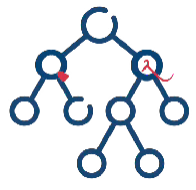
\includegraphics[height=0.9cm]{msca_logo.png}}%
  \end{center}
  \vspace{0.45cm}
  \begin{center}
    \begin{minipage}{0.1\textwidth}\centering
      \href{https://quantlet.com}{
\includegraphics[height=0.9cm]{ql_logo.png}}\end{minipage}%
    \begin{minipage}{0.78\textwidth}\centering
      {\Large\bfseries\usebeamercolor[fg]{title}\inserttitle}\par\vspace{0.25cm}
      {\large\usebeamercolor[fg]{title}\insertsubtitle}\end{minipage}%
    \begin{minipage}{0.1\textwidth}\centering
      \href{https://quantinar.com}{
\includegraphics[height=0.9cm]{qr_logo.png}}\end{minipage}
  \end{center}
  \vfill
  \hspace{0.4cm}{\bfseries\insertauthor}\par\vspace{0.12cm}
  \hspace{0.4cm}\begin{minipage}[t]{0.92\textwidth}\raggedright\footnotesize\insertinstitute\end{minipage}
  \par\vspace{0.4cm}}

% ---------------------------------------------------------------- lecture metadata
\newcommand{\nnshort}{}
\newcommand{\nnnb}{notebooks}
\newcommand{\nnrepo}{https://github.com/danpele/NEURAL_BIZ/tree/main}
% language-dependent labels (English default; \nnromanian switches to Romanian, call it before \nnlecture)
\newcommand{\txtcourse}{Neural Networks and Deep Learning}
\newcommand{\txtlecture}{Lecture}
\newcommand{\txtoutline}{Outline}
\newcommand{\txtintuition}{In one sentence:}
\newcommand{\txtjob}{In practice:}
\newcommand{\txttry}{Experiment yourself:}
\newcommand{\txtwhere}{where}
\newcommand{\txtsim}{SIMULATED DATA (teaching illustration)}
\newcommand{\txtnbsuffix}{}
\newcommand{\txtinstitute}{Bucharest University of Economic Studies (ASE), Department of Statistics and Econometrics\\
    Romanian Academy, Institute for Economic Forecasting (IPE)\\
    IDA Institute Digital Assets \textbullet\ AI4EFin \textbullet\ MSCA Digital Finance}
\newcommand{\nnromanian}{%
  \renewcommand{\txtcourse}{Rețele neuronale și deep learning}%
  \renewcommand{\txtlecture}{Cursul}%
  \renewcommand{\txtoutline}{Cuprins}%
  \renewcommand{\txtintuition}{Pe scurt:}%
  \renewcommand{\txtjob}{În practică:}%
  \renewcommand{\txttry}{Exercițiu practic:}%
  \renewcommand{\txtwhere}{unde}%
  \renewcommand{\txtsim}{DATE SIMULATE (doar pentru ilustrare)}%
  \renewcommand{\txtnbsuffix}{\string_ro}%
  \renewcommand{\txtinstitute}{Academia de Studii Economice din București (ASE), Departamentul de Statistică și Econometrie\\
    Academia Română, Institutul de Prognoză Economică (IPE)\\
    IDA Institute Digital Assets \textbullet\ AI4EFin \textbullet\ MSCA Digital Finance}}
\newcommand{\nnlecture}[2]{%
  \renewcommand{\nnshort}{\txtlecture\ #1}%
  \renewcommand{\nnnb}{notebooks/L#1\string_notebook\txtnbsuffix.ipynb}%
  \title[NN]{\txtcourse}%
  \subtitle{\txtlecture\ #1: #2}%
  \author{Prof.\ dr.\ Daniel Traian PELE}%
  \institute{\txtinstitute}%
  \date{}}

% ---------------------------------------------------------------- teaching blocks (one message per frame)
% \intuition{one plain sentence}  ->  formula with every symbol defined  ->  real-data example  ->  \manager{one line}
\newcommand{\intuition}[1]{\begin{itemize}\item {\color{MainBlue}\textbf{\txtintuition}}~#1\end{itemize}\vspace{0.6mm}}
\newcommand{\manager}[1]{\colorbox{Forest!10}{\parbox{\dimexpr\linewidth-2\fboxsep\relax}{\footnotesize
  \begin{itemize}\setlength{\itemsep}{0pt}\item \textbf{\color{Forest}\txtjob}~#1\end{itemize}}}}
% Experiment yourself: pointer to the matching notebook section
\newcommand{\tryit}[1]{{\scriptsize\href{\nnrepo/\nnnb}{%
  \raisebox{-0.15em}{
\includegraphics[height=0.85em]{ql_logo.png}}\,\textbf{\txttry}~\color{MainBlue}#1}}}
% bottom row: manager line (left) + experiment pointer (right), pinned to the bottom of the frame
\newcommand{\bottomrow}[2]{\par\vfill\noindent\begin{minipage}[b]{0.72\linewidth}#1\end{minipage}\hfill
  \begin{minipage}[b]{0.26\linewidth}\raggedleft #2\end{minipage}\par\vspace{0.5mm}}
\newcommand{\where}[1]{{\footnotesize\textbf{\txtwhere}~#1\par}}

% ---------------------------------------------------------------- helpers
% chart source line under a figure: \chartsource{Source ...; period ...}
\newcommand{\chartsource}[1]{\par\vspace{1pt}{\scriptsize\color{FooterGray}#1\par}}
% link to code: \quantlet{label}{path inside the repo}
\newcommand{\quantlet}[2]{\par\vspace{1pt}\hfill\href{\nnrepo/#2}{%
  \raisebox{-0.15em}{
\includegraphics[height=0.75em]{ql_logo.png}}\textcolor{MainBlue}{\scriptsize\ #1}}}
% inline Quantlet link for the bottom-right corner of a frame: \qlink{label}{path inside the repo}
\newcommand{\qlink}[2]{{\scriptsize\href{\nnrepo/#2}{\raisebox{-0.15em}{
\includegraphics[height=0.85em]{ql_logo.png}}\,\textcolor{MainBlue}{#1}}}}
\newcommand{\simlabel}{\colorbox{Crimson!12}{\scriptsize\bfseries\color{Crimson}\txtsim}}
\newcommand{\E}{\mathbb{E}}
\newcommand{\Var}{\operatorname{Var}}
\newcommand{\Cov}{\operatorname{Cov}}
\newcommand{\Corr}{\operatorname{Corr}}
\newcommand{\asinh}{\operatorname{asinh}}
\newcommand{\iid}{\overset{\text{i.i.d.}}{\sim}}
\newcommand{\EUR}{EUR}
% deep-learning notation (Bishop & Bishop, 2024): vectors bold lower case, matrices bold upper case
\newcommand{\R}{\mathbb{R}}
\newcommand{\vx}{\mathbf{x}}
\newcommand{\vy}{\mathbf{y}}
\newcommand{\vz}{\mathbf{z}}
\newcommand{\vh}{\mathbf{h}}
\newcommand{\vw}{\mathbf{w}}
\newcommand{\vb}{\mathbf{b}}
\newcommand{\mW}{\mathbf{W}}
\newcommand{\mX}{\mathbf{X}}
\newcommand{\btheta}{\boldsymbol{\theta}}
\newcommand{\loss}{\mathcal{L}}
\newcommand{\dataset}{\mathcal{D}}
\DeclareMathOperator*{\argmin}{arg\,min}
\DeclareMathOperator*{\argmax}{arg\,max}
\DeclareMathOperator{\softmax}{softmax}
\DeclareMathOperator{\ReLU}{ReLU}
\DeclareMathOperator{\sigm}{\sigma}

%   \nnlecture{k}{Lecture title}
% Logos live in lectures/common/logos/, charts in lectures/Lk/charts/.
% Do NOT add \hfuzz / \vfuzz / \hbadness here: overfull boxes must be fixed, not hidden.
% =============================================================================

\usetheme{default}
\setbeamersize{text margin left=7mm, text margin right=7mm}

% ---------------------------------------------------------------- packages
\usepackage[utf8]{inputenc}
\usepackage[T1]{fontenc}
\usepackage{lmodern}
\usepackage{amsmath, amssymb}
\usepackage{mathtools}
\usepackage{bm}
\usepackage{tikz}
\usetikzlibrary{arrows.meta, positioning, calc, shapes.misc}
\usepackage{booktabs}
\usepackage{array}
\usepackage{graphicx}
\usepackage{colortbl}
\usepackage{xcolor}
\usepackage{multicol}
\hypersetup{colorlinks=true, linkcolor=MainBlue, urlcolor=MainBlue, citecolor=MainBlue}
\graphicspath{{../common/logos/}}   % charts are included with their language folder: charts/en/, charts/ro/

% ---------------------------------------------------------------- colours
\definecolor{MainBlue}{RGB}{26, 58, 110}
\definecolor{IDAred}{RGB}{205, 0, 0}
\definecolor{DarkGray}{RGB}{51, 51, 51}
\definecolor{FooterGray}{RGB}{100, 100, 100}
\definecolor{BlockGray}{RGB}{236, 238, 242}
\definecolor{KeynoteGray}{RGB}{218, 218, 218}
\definecolor{Crimson}{RGB}{190, 40, 50}
\definecolor{Forest}{RGB}{30, 110, 50}
\definecolor{Bitter}{RGB}{214, 150, 20}
% chart palette (same hex values and order as lectures/common/nn_plot.py SERIES)
\definecolor{Ser1}{HTML}{2A78D6}
\definecolor{Ser2}{HTML}{EB6834}
\definecolor{Ser3}{HTML}{1BAF7A}
\definecolor{Ser4}{HTML}{EDA100}
\definecolor{Ser5}{HTML}{E87BA4}
\definecolor{Ser6}{HTML}{008300}
\definecolor{Ser7}{HTML}{6250D6}
\definecolor{Ser8}{HTML}{E34948}

\setbeamertemplate{background}{%
  \begin{tikzpicture}[remember picture, overlay]
    \shade[shading=axis, shading angle=315, top color=white, bottom color=KeynoteGray]
      (current page.south west) rectangle (current page.north east);
  \end{tikzpicture}}
\setbeamercolor{background canvas}{bg=}
\setbeamercolor{structure}{fg=MainBlue}
\setbeamercolor{normal text}{fg=DarkGray}
\setbeamercolor{title}{fg=IDAred}
\setbeamercolor{frametitle}{fg=IDAred, bg=}
\setbeamercolor{block title}{bg=MainBlue, fg=white}
\setbeamercolor{block body}{bg=BlockGray, fg=DarkGray}
\setbeamercolor{block title alerted}{bg=Crimson, fg=white}
\setbeamercolor{block body alerted}{bg=Crimson!7, fg=DarkGray}
\setbeamercolor{block title example}{bg=Forest, fg=white}
\setbeamercolor{block body example}{bg=Forest!7, fg=DarkGray}
\setbeamercolor{item}{fg=MainBlue}
\setbeamerfont{frametitle}{size=\large, series=\bfseries}
\setbeamerfont{block title}{size=\small, series=\bfseries}
\setbeamertemplate{blocks}[rounded][shadow=false]
\setbeamertemplate{itemize item}{\color{MainBlue}$\boxdot$}
\setbeamertemplate{itemize subitem}{\color{MainBlue}\scriptsize$\blacktriangleright$}
% compact two-level lists: level 1 = main point, level 2 = details (no text outside bullets)
\setbeamerfont{itemize/enumerate subbody}{size=\footnotesize}
\setlength{\leftmargini}{1.1em}
\setlength{\leftmarginii}{1.1em}
\setbeamertemplate{itemize/enumerate body begin}{\setlength{\topsep}{0pt}\setlength{\partopsep}{0pt}\setlength{\parskip}{0pt}}
\setbeamertemplate{itemize/enumerate subbody begin}{\setlength{\topsep}{0pt}\setlength{\partopsep}{0pt}\setlength{\itemsep}{0pt}\vspace{-0.4ex}}

\setbeamertemplate{enumerate item}{\color{MainBlue}\insertenumlabel.}
\setlength{\leftmargini}{1.3em}
\setlength{\leftmarginii}{1.2em}
\setbeamertemplate{navigation symbols}{}
\setbeamertemplate{section in toc}{\color{MainBlue}$\blacktriangleright$~\inserttocsection}
\setbeamertemplate{caption}{\raggedright\insertcaption\par}
% frame subtitle = precise citation line under the claim title (Weron style)
\setbeamerfont{framesubtitle}{size=\footnotesize}
\setbeamercolor{framesubtitle}{fg=FooterGray}
% outline that reappears at every section with the current section highlighted
\setbeamertemplate{section in toc shaded}[default][35]
\setbeamertemplate{subsection in toc shaded}[default][35]
\setbeamertemplate{subsection in toc}{\leavevmode\leftskip=2.2em\color{DarkGray}\small\inserttocsubsection\par}
\AtBeginSection[]{{\begin{frame}{\txtoutline}\vspace{2mm}\small
  \tableofcontents[currentsection,hideothersubsections]\end{frame}}}

% ---------------------------------------------------------------- head and foot
\setbeamertemplate{headline}{%
  \vskip10pt%
  \hbox to \paperwidth{\hskip0.5cm%
    {\small\color{FooterGray}\renewcommand{\hyperlink}[2]{##2}\insertsectionhead}%
    \hfill\textcolor{FooterGray}{\small\insertframenumber}\hskip0.5cm}%
  \vskip4pt{\color{FooterGray}\hrule height 0.4pt}}
% footer as in the other courses (MFM, SFM): course name on the left, small sparkline on the right
\setbeamertemplate{footline}{%
  {\color{FooterGray}\hrule height 0.4pt}\vskip4pt%
  \hbox to \paperwidth{\hskip0.5cm%
    \textcolor{FooterGray}{\small\txtcourse}%
    \hfill\raisebox{-0.1em}{\begin{tikzpicture}[x=0.08em, y=0.08em, line width=0.4pt]
      \draw[FooterGray] (0,3) -- (1,4) -- (2,3.5) -- (3,5) -- (4,4) -- (5,6) -- (6,5.5) -- (7,4) -- (8,5) -- (9,7) -- (10,6) -- (11,5) -- (12,6.5) -- (13,8) -- (14,7) -- (15,6) -- (16,7.5) -- (17,9) -- (18,8) -- (19,7) -- (20,8.5) -- (21,10) -- (22,9) -- (23,8) -- (24,9.5);
    \end{tikzpicture}}\hskip0.5cm}%
  \vskip6pt}

% ---------------------------------------------------------------- title page
\defbeamertemplate*{title page}{nn}[1][]{%
  \vspace{0.15cm}
  \begin{center}
    \href{https://www.ase.ro}{
\includegraphics[height=0.9cm]{ase_logo.png}}\hspace{0.3cm}%
    \href{https://ipe.ro/new}{
\includegraphics[height=0.9cm]{acad_logo.png}}\hspace{0.3cm}%
    \href{https://theida.net}{
\includegraphics[height=0.9cm]{ida_logo.png}}\hspace{0.3cm}%
    \href{https://blockchain-research-center.com}{
\includegraphics[height=0.9cm]{brc_logo.png}}\hspace{0.3cm}%
    \href{https://www.ai4efin.ase.ro}{
\includegraphics[height=0.9cm]{ai4efin_logo.png}}\hspace{0.3cm}%
    \href{https://www.digital-finance-msca.com}{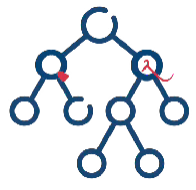
\includegraphics[height=0.9cm]{msca_logo.png}}%
  \end{center}
  \vspace{0.45cm}
  \begin{center}
    \begin{minipage}{0.1\textwidth}\centering
      \href{https://quantlet.com}{
\includegraphics[height=0.9cm]{ql_logo.png}}\end{minipage}%
    \begin{minipage}{0.78\textwidth}\centering
      {\Large\bfseries\usebeamercolor[fg]{title}\inserttitle}\par\vspace{0.25cm}
      {\large\usebeamercolor[fg]{title}\insertsubtitle}\end{minipage}%
    \begin{minipage}{0.1\textwidth}\centering
      \href{https://quantinar.com}{
\includegraphics[height=0.9cm]{qr_logo.png}}\end{minipage}
  \end{center}
  \vfill
  \hspace{0.4cm}{\bfseries\insertauthor}\par\vspace{0.12cm}
  \hspace{0.4cm}\begin{minipage}[t]{0.92\textwidth}\raggedright\footnotesize\insertinstitute\end{minipage}
  \par\vspace{0.4cm}}

% ---------------------------------------------------------------- lecture metadata
\newcommand{\nnshort}{}
\newcommand{\nnnb}{notebooks}
\newcommand{\nnrepo}{https://github.com/danpele/NEURAL_BIZ/tree/main}
% language-dependent labels (English default; \nnromanian switches to Romanian, call it before \nnlecture)
\newcommand{\txtcourse}{Neural Networks and Deep Learning}
\newcommand{\txtlecture}{Lecture}
\newcommand{\txtoutline}{Outline}
\newcommand{\txtintuition}{In one sentence:}
\newcommand{\txtjob}{In practice:}
\newcommand{\txttry}{Experiment yourself:}
\newcommand{\txtwhere}{where}
\newcommand{\txtsim}{SIMULATED DATA (teaching illustration)}
\newcommand{\txtnbsuffix}{}
\newcommand{\txtinstitute}{Bucharest University of Economic Studies (ASE), Department of Statistics and Econometrics\\
    Romanian Academy, Institute for Economic Forecasting (IPE)\\
    IDA Institute Digital Assets \textbullet\ AI4EFin \textbullet\ MSCA Digital Finance}
\newcommand{\nnromanian}{%
  \renewcommand{\txtcourse}{Rețele neuronale și deep learning}%
  \renewcommand{\txtlecture}{Cursul}%
  \renewcommand{\txtoutline}{Cuprins}%
  \renewcommand{\txtintuition}{Pe scurt:}%
  \renewcommand{\txtjob}{În practică:}%
  \renewcommand{\txttry}{Exercițiu practic:}%
  \renewcommand{\txtwhere}{unde}%
  \renewcommand{\txtsim}{DATE SIMULATE (doar pentru ilustrare)}%
  \renewcommand{\txtnbsuffix}{\string_ro}%
  \renewcommand{\txtinstitute}{Academia de Studii Economice din București (ASE), Departamentul de Statistică și Econometrie\\
    Academia Română, Institutul de Prognoză Economică (IPE)\\
    IDA Institute Digital Assets \textbullet\ AI4EFin \textbullet\ MSCA Digital Finance}}
\newcommand{\nnlecture}[2]{%
  \renewcommand{\nnshort}{\txtlecture\ #1}%
  \renewcommand{\nnnb}{notebooks/L#1\string_notebook\txtnbsuffix.ipynb}%
  \title[NN]{\txtcourse}%
  \subtitle{\txtlecture\ #1: #2}%
  \author{Prof.\ dr.\ Daniel Traian PELE}%
  \institute{\txtinstitute}%
  \date{}}

% ---------------------------------------------------------------- teaching blocks (one message per frame)
% \intuition{one plain sentence}  ->  formula with every symbol defined  ->  real-data example  ->  \manager{one line}
\newcommand{\intuition}[1]{\begin{itemize}\item {\color{MainBlue}\textbf{\txtintuition}}~#1\end{itemize}\vspace{0.6mm}}
\newcommand{\manager}[1]{\colorbox{Forest!10}{\parbox{\dimexpr\linewidth-2\fboxsep\relax}{\footnotesize
  \begin{itemize}\setlength{\itemsep}{0pt}\item \textbf{\color{Forest}\txtjob}~#1\end{itemize}}}}
% Experiment yourself: pointer to the matching notebook section
\newcommand{\tryit}[1]{{\scriptsize\href{\nnrepo/\nnnb}{%
  \raisebox{-0.15em}{
\includegraphics[height=0.85em]{ql_logo.png}}\,\textbf{\txttry}~\color{MainBlue}#1}}}
% bottom row: manager line (left) + experiment pointer (right), pinned to the bottom of the frame
\newcommand{\bottomrow}[2]{\par\vfill\noindent\begin{minipage}[b]{0.72\linewidth}#1\end{minipage}\hfill
  \begin{minipage}[b]{0.26\linewidth}\raggedleft #2\end{minipage}\par\vspace{0.5mm}}
\newcommand{\where}[1]{{\footnotesize\textbf{\txtwhere}~#1\par}}

% ---------------------------------------------------------------- helpers
% chart source line under a figure: \chartsource{Source ...; period ...}
\newcommand{\chartsource}[1]{\par\vspace{1pt}{\scriptsize\color{FooterGray}#1\par}}
% link to code: \quantlet{label}{path inside the repo}
\newcommand{\quantlet}[2]{\par\vspace{1pt}\hfill\href{\nnrepo/#2}{%
  \raisebox{-0.15em}{
\includegraphics[height=0.75em]{ql_logo.png}}\textcolor{MainBlue}{\scriptsize\ #1}}}
% inline Quantlet link for the bottom-right corner of a frame: \qlink{label}{path inside the repo}
\newcommand{\qlink}[2]{{\scriptsize\href{\nnrepo/#2}{\raisebox{-0.15em}{
\includegraphics[height=0.85em]{ql_logo.png}}\,\textcolor{MainBlue}{#1}}}}
\newcommand{\simlabel}{\colorbox{Crimson!12}{\scriptsize\bfseries\color{Crimson}\txtsim}}
\newcommand{\E}{\mathbb{E}}
\newcommand{\Var}{\operatorname{Var}}
\newcommand{\Cov}{\operatorname{Cov}}
\newcommand{\Corr}{\operatorname{Corr}}
\newcommand{\asinh}{\operatorname{asinh}}
\newcommand{\iid}{\overset{\text{i.i.d.}}{\sim}}
\newcommand{\EUR}{EUR}
% deep-learning notation (Bishop & Bishop, 2024): vectors bold lower case, matrices bold upper case
\newcommand{\R}{\mathbb{R}}
\newcommand{\vx}{\mathbf{x}}
\newcommand{\vy}{\mathbf{y}}
\newcommand{\vz}{\mathbf{z}}
\newcommand{\vh}{\mathbf{h}}
\newcommand{\vw}{\mathbf{w}}
\newcommand{\vb}{\mathbf{b}}
\newcommand{\mW}{\mathbf{W}}
\newcommand{\mX}{\mathbf{X}}
\newcommand{\btheta}{\boldsymbol{\theta}}
\newcommand{\loss}{\mathcal{L}}
\newcommand{\dataset}{\mathcal{D}}
\DeclareMathOperator*{\argmin}{arg\,min}
\DeclareMathOperator*{\argmax}{arg\,max}
\DeclareMathOperator{\softmax}{softmax}
\DeclareMathOperator{\ReLU}{ReLU}
\DeclareMathOperator{\sigm}{\sigma}

\usepackage[romanian]{babel}
\nnromanian
\nnlecture{12}{Modele lingvistice mari în finanțe și formularea instrucțiunilor (prompt engineering)}
\begin{document}
{\setbeamertemplate{headline}{}\setbeamertemplate{footline}{}
\begin{frame}\titlepage\end{frame}}
% END-FRONT-MATTER

\begin{frame}{Obiectivele cursului}
\small
\begin{itemize}\setlength{\itemsep}{4pt}
  \item Să scrieți obiectivul unui model de limbaj, perplexitatea și temperatura de eșantionare și să le măsurați pe discursuri ale unei bănci centrale.
  \item Să explicați preantrenarea, ajustarea pe instrucțiuni și alinierea la preferințele umane, cu funcțiile lor de pierdere.
  \item Să transformați un prompt într-un clasificator și să evaluați prompturile zero-shot, few-shot și chain-of-thought pe texte financiare etichetate, cu intervale de încredere.
  \item Să construiți și să evaluați generarea augmentată prin regăsire (RAG) pe discursuri reale și să măsurați halucinațiile.
  \item Să testați retrospectiv un model de limbaj folosit pentru valoarea expusă la risc (VaR) și să cunoașteți riscurile: scurgerea de date, costul, calibrarea.
\end{itemize}
\end{frame}

% BEGIN-ABBR

\begin{frame}{Abrevieri}
\small
\vspace{-1mm}\begin{columns}[T,onlytextwidth]
\begin{column}{0.49\textwidth}{\scriptsize\renewcommand{\arraystretch}{0.96}\begin{tabular}{@{}>{\bfseries}l@{\ \ }p{0.74\linewidth}@{}}AI & inteligență artificială\\
API & interfață de programare a aplicațiilor\\
ASE & Academia de Studii Economice din București\\
BCE & Banca Centrală Europeană\\
BERT & reprezentări bidirecționale ale codificatorului transformer\\
BM25 & funcția de ordonare Best Matching 25\\
BPE & codificare prin perechi de octeți (byte-pair encoding)\\
DPO & optimizarea directă a preferințelor\\
ECE & eroarea de calibrare așteptată\\
ES & pierderea așteptată în coada distribuției (expected shortfall)\\
FinBERT & model BERT adaptat textelor financiare\\
GARCH & heteroscedasticitate condiționată autoregresivă generalizată\\
GPT & transformer generativ preantrenat\\\end{tabular}}\end{column}
\begin{column}{0.49\textwidth}{\scriptsize\renewcommand{\arraystretch}{0.96}\begin{tabular}{@{}>{\bfseries}l@{\ \ }p{0.74\linewidth}@{}}HS & simulare istorică\\
IPE & Institutul de Prognoză Economică, Academia Română\\
KL & divergența Kullback--Leibler\\
LLM & model lingvistic mare\\
LoRA & adaptare de rang mic (low-rank adaptation)\\
LR & raportul de verosimilitate\\
MRR & rangul reciproc mediu\\
RAG & generare augmentată prin regăsire (retrieval-augmented generation)\\
RLHF & învățare prin recompensă din feedback uman\\
SFT & ajustare fină supervizată\\
TF-IDF & frecvența termenului--frecvența inversă în documente\\
UE & Uniunea Europeană\\
VaR & valoarea expusă la risc (Value-at-Risk)\\\end{tabular}}\end{column}
\end{columns}
\end{frame}

% END-ABBR


\section{De la prezicerea următorului token la modelele lingvistice mari}

\begin{frame}{Datele de tip text în instituțiile financiare}
\small
\begin{itemize}\setlength{\itemsep}{3pt}
  \item \textbf{Piețe}
    \begin{itemize}\setlength{\itemsep}{0pt}
      \item Știrile și rețelele sociale mișcă prețurile în cîteva minute; sentimentul este un semnal
    \end{itemize}
  \item \textbf{Bănci centrale}
    \begin{itemize}\setlength{\itemsep}{0pt}
      \item Discursurile și minutele ghidează așteptările privind dobînzile; în datele noastre, Banca Centrală Europeană (BCE) are 400 de discursuri din 2022
    \end{itemize}
  \item \textbf{Credit și risc}
    \begin{itemize}\setlength{\itemsep}{0pt}
      \item Dosare de credit, rapoarte anuale, rapoarte de risc: citirea lor costă ore de analiză
    \end{itemize}
  \item \textbf{Acest curs}
    \begin{itemize}\setlength{\itemsep}{0pt}
      \item Modele lingvistice mari (LLM) deschise, rulate pe un laptop, evaluate pe date etichetate, niciodată acceptate fără verificare
    \end{itemize}
\end{itemize}
\end{frame}

\begin{frame}{Modelul de limbaj: probabilitatea următorului token, prin entropie încrucișată}
\footnotesize
\intuition{tot ce face un LLM, de la răspunsuri la cod, este prezicerea repetată a următorului token.}
\begin{columns}[T,onlytextwidth]
\begin{column}{0.62\textwidth}
\[ p_{\btheta}(x_1,\dots,x_T)=\prod_{t=1}^{T}p_{\btheta}(x_t\mid x_{<t}) \]\[ \loss(\btheta)=-\frac{1}{T}\sum_{t=1}^{T}\log p_{\btheta}(x_t\mid x_{<t}),\quad \mathrm{PPL}=e^{\loss} \]{\footnotesize\begin{itemize}\setlength{\itemsep}{0pt}
  \item \textbf{\txtwhere}
    \begin{itemize}\setlength{\itemsep}{0pt}
      \item $x_t$ = tokenul $t$
      \item $p_{\btheta}$ = softmax peste vocabular (transformer cauzal, cursul 7)
      \item Perplexitatea = numărul efectiv de tokeni următori echiprobabili.
    \end{itemize}
\end{itemize}\par}
\end{column}
\begin{column}{0.35\textwidth}
\begin{itemize}\setlength{\itemsep}{2pt}
  \item \textbf{Discursuri BCE} după iulie 2025: perplexitatea 14{,}71 (0,5B), 10{,}63 (1,5B), 9{,}43 (3B).
\end{itemize}
\end{column}
\end{columns}
\par\vfill\manager{o perplexitate mai mică pe documentele proprii înseamnă că modelul „vorbește” limbajul domeniului.}\par\vspace{0.5mm}
\par\vfill\noindent{\scriptsize\color{FooterGray}(Bishop \& Bishop, 2024, ch.\ 12)}\hfill\tryit{notebook \S1}\par\vspace{0.5mm}
\end{frame}

\begin{frame}{Tokenii sînt fragmente de cuvinte: codificarea byte-pair}
\footnotesize
\intuition{cuvintele frecvente sînt un singur token, iar cele rare și numerele se împart; modelul nu vede litere, doar indici de tokeni.}
\begin{columns}[T,onlytextwidth]
\begin{column}{0.53\textwidth}
\[ (a,b)^{*}=\argmax_{(a,b)}\ \mathrm{count}(a\,b)\ \Rightarrow\ \text{unește}\ a\,b\to ab \]{\footnotesize\begin{itemize}\setlength{\itemsep}{0pt}
  \item \textbf{\txtwhere}
    \begin{itemize}\setlength{\itemsep}{0pt}
      \item Se repetă pînă cînd vocabularul este complet: codificarea byte-pair (BPE), 151\,665 de tokeni în Qwen2.5
      \item WordPiece, 30\,522 de tokeni într-un model de reprezentări bidirecționale ale codificatorului transformer (BERT) adaptat finanțelor (FinBERT).
    \end{itemize}
\end{itemize}\par}
\end{column}
\begin{column}{0.44\textwidth}
\begin{itemize}\setlength{\itemsep}{2pt}
  \item \textbf{Exemplu} (20 tokeni): - |  Cash |  flow |  from |  operating |  activities |  before |  investments |  was |  EUR |   | 0 | . | 8 |  - | 1 | . | 2 |  million |  ..
  \item \textbf{Financial PhraseBank}: 1{,}35 tokeni Qwen și 1{,}24 tokeni WordPiece pe cuvînt.
\end{itemize}
\end{column}
\end{columns}
\par\vfill\manager{costul și limita contextului se măsoară în tokeni, nu în cuvinte: socotiți aproximativ 1,3 tokeni pe cuvînt în engleză.}\par\vspace{0.5mm}
\par\vfill\noindent{\scriptsize\color{FooterGray}(Sennrich, Haddow \& Birch, 2016)}\hfill\tryit{notebook \S1}\par\vspace{0.5mm}
\end{frame}

\begin{frame}{Lungimea propozițiilor în cuvinte și în tokeni: două metode de tokenizare}
\small
\intuition{aceleași 4\,838 propoziții sînt puțin mai lungi în tokeni decît în cuvinte.}
\begin{center}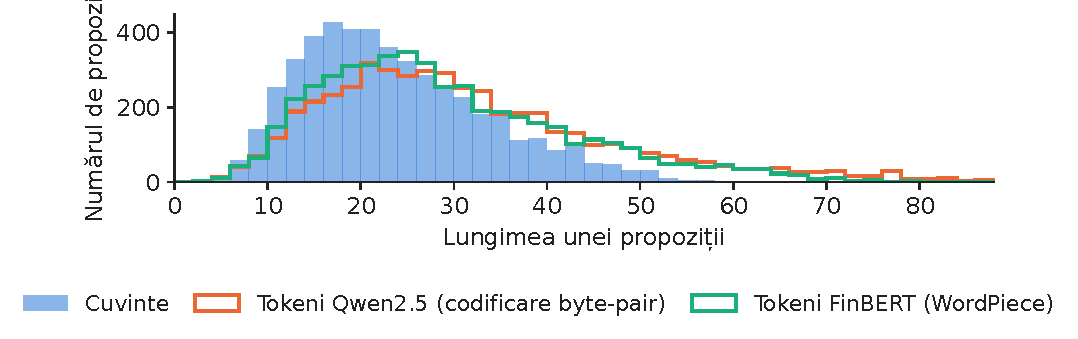
\includegraphics[width=\textwidth,height=0.550\textheight,keepaspectratio]{charts/ro/tokens_per_sentence.pdf}\end{center}\vspace{-3mm}
\chartsource{Sursa: Financial PhraseBank (Malo et al., 2014). Date: 4.838 de propoziții.}
\vspace{0.5mm}
\begin{itemize}\setlength{\itemsep}{0pt}
  \item Media: 23{,}1 cuvinte, 31{,}1 tokeni Qwen, 28{,}6 tokeni WordPiece
    \begin{itemize}\setlength{\itemsep}{0pt}
      \item Un discurs BCE are în medie 4\,143 de tokeni (cel mai lung: 22\,897).
    \end{itemize}
\end{itemize}
\par\vfill\noindent{\scriptsize\color{FooterGray}}\hfill\qlink{NN\_L12\_tokens\_per\_sentence}{Quantlets/L12/NN_L12_tokens_per_sentence}\par\vspace{0.5mm}
\end{frame}

\begin{frame}{Temperatura schimbă forma distribuției următorului token}
\footnotesize
\intuition{modelul produce scoruri (logits); temperatura decide cît de îndrăzneț eșantionăm din ele.}
\begin{columns}[T,onlytextwidth]
\begin{column}{0.5\textwidth}
\[ p_T(v\mid x_{<t})=\frac{\exp(z_v/T)}{\sum_{u}\exp(z_u/T)} \]\[ H_T=-\sum_v p_T(v)\log p_T(v) \]{\footnotesize\begin{itemize}\setlength{\itemsep}{0pt}
  \item \textbf{\txtwhere}
    \begin{itemize}\setlength{\itemsep}{0pt}
      \item $z_v$ = scorul (logit) tokenului $v$
      \item $T\to 0$: mereu tokenul cel mai probabil (lacom)
      \item $T>1$: distribuție mai plată, mai diversă, cu mai multe erori
      \item $H_T$ = entropia, în nats.
    \end{itemize}
\end{itemize}\par}
\end{column}
\begin{column}{0.47\textwidth}
\begin{itemize}\setlength{\itemsep}{2pt}
  \item \textbf{Prompt} din discursul BCE din 30 octombrie 2026: „The inflation impact is limited: \ldots”
  \item \textbf{Primul token} „the”: 49{,}9\,\% la $T$ = 0,5, 10{,}1\,\% la 1, 0{,}4\,\% la 2
    \begin{itemize}\setlength{\itemsep}{0pt}
      \item Entropia 1{,}74, 6{,}20, 10{,}29.
    \end{itemize}
\end{itemize}
\end{column}
\end{columns}
\par\vfill\manager{pentru clasificare și extragere folosiți temperatura 0
    \begin{itemize}\setlength{\itemsep}{0pt}
      \item Temperaturile mari sînt pentru generarea de idei.
    \end{itemize}}\par\vspace{0.5mm}
\par\vfill\noindent{\scriptsize\color{FooterGray}}\hfill\tryit{notebook \S2}\par\vspace{0.5mm}
\end{frame}

\begin{frame}{Probabilitățile următorului token: un model real, o frază reală}
\small
\intuition{la temperatură mică aproape toată masa de probabilitate stă pe o continuare; la temperatură mare, tokenii improbabili devin plauzibili.}
\begin{center}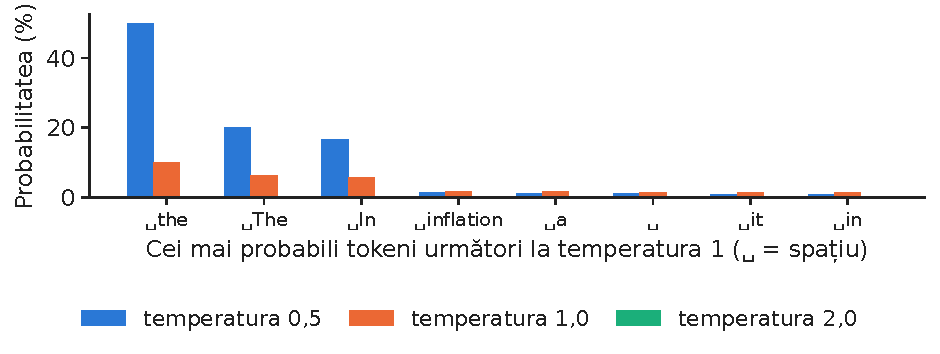
\includegraphics[width=\textwidth,height=0.584\textheight,keepaspectratio]{charts/ro/next_token.pdf}\end{center}\vspace{-3mm}
\chartsource{Sursa: Banca Centrală Europeană, setul de discursuri. Date: începutul unei fraze din discursul BCE din 30 octombrie 2026; modelul Qwen2.5-1.5B-Instruct.}
\par\vfill\noindent{\scriptsize\color{FooterGray}}\hfill\qlink{NN\_L12\_next\_token}{Quantlets/L12/NN_L12_next_token}\par\vspace{0.5mm}
\end{frame}

\begin{frame}{Scalarea: modelele mai mari prezic mai bine textul, după o lege de putere}
\footnotesize
\intuition{pierderea scade ca o putere a numărului de parametri și de tokeni de antrenare.}
\begin{columns}[T,onlytextwidth]
\begin{column}{0.53\textwidth}
\[ \loss(P,D)=E+\frac{A}{P^{\alpha}}+\frac{B}{D^{\beta}} \]\[ \text{estimare proprie:}\ \log\loss=a+b\log P,\quad \hat b=\ensuremath{-}0{,}100 \]{\footnotesize\begin{itemize}\setlength{\itemsep}{0pt}
  \item \textbf{\txtwhere}
    \begin{itemize}\setlength{\itemsep}{0pt}
      \item $P$ = numărul de parametri
      \item $D$ = tokenii de antrenare
      \item $E$ = pierderea ireductibilă
      \item $\alpha,\beta\approx 0{,}3$ (Hoffmann et al., 2022)
      \item $\hat b$ din cele trei dimensiuni Qwen2.5, pe discursurile BCE de după iulie 2025.
    \end{itemize}
\end{itemize}\par}
\end{column}
\begin{column}{0.44\textwidth}
\begin{itemize}\setlength{\itemsep}{2pt}
  \item \textbf{Trei puncte nu fac o lege}: panta descrie eșantionul nostru, nu este o prognoză.
  \item \textbf{Optimul de calcul}: aproximativ 20 de tokeni de antrenare pe parametru.
\end{itemize}
\end{column}
\end{columns}
\par\vfill\manager{un model de 3B pe laptop nu costă nimic pe apel
    \begin{itemize}\setlength{\itemsep}{0pt}
      \item Un model de vîrf costă pe token: măsurați întîi cîștigul.
    \end{itemize}}\par\vspace{0.5mm}
\par\vfill\noindent{\scriptsize\color{FooterGray}(Kaplan et al., 2020; Hoffmann et al., 2022)}\hfill\tryit{notebook \S1}\par\vspace{0.5mm}
\end{frame}

\begin{frame}{Discursurile mai vechi par mai ușoare: un avertisment despre limita datelor de antrenare}
\small
\intuition{textul pe care modelul l-ar fi putut vedea la preantrenare are o perplexitate mai mică decît textul scris după aceea.}
\begin{center}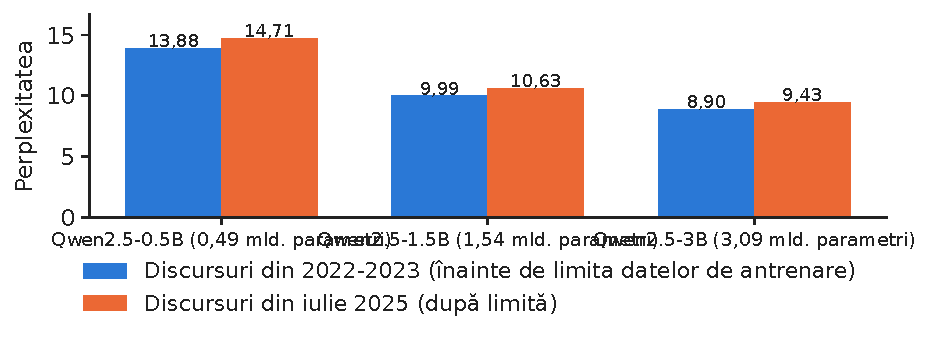
\includegraphics[width=\textwidth,height=0.196\textheight,keepaspectratio]{charts/ro/perplexity_size.pdf}\end{center}\vspace{-3mm}
\chartsource{Sursa: Banca Centrală Europeană, setul de discursuri. Date: 40 + 40 de discursuri, primii 1.024 de tokeni din fiecare.}
\vspace{0.5mm}
\begin{itemize}\setlength{\itemsep}{0pt}
  \item 3B: 8{,}90 pe discursurile din 2022--2023, față de 9{,}43 după iulie 2025
    \begin{itemize}\setlength{\itemsep}{0pt}
      \item Mai mică pentru discursurile vechi la toate dimensiunile.
    \end{itemize}
  \item Și temele s-au schimbat
    \begin{itemize}\setlength{\itemsep}{0pt}
      \item Diferența este un simptom, nu o dovadă, a memorării.
    \end{itemize}
\end{itemize}
\par\vfill\manager{evaluați un LLM pe documente scrise după limita datelor sale de antrenare
    \begin{itemize}\setlength{\itemsep}{0pt}
      \item Altfel scorul poate fi umflat prin scurgerea datelor.
    \end{itemize}}\par\vspace{0.5mm}
\par\vfill\noindent{\scriptsize\color{FooterGray}}\hfill\qlink{NN\_L12\_perplexity\_size}{Quantlets/L12/NN_L12_perplexity_size}\par\vspace{0.5mm}
\end{frame}


\section{Preantrenare, ajustare pe instrucțiuni și aliniere}

\begin{frame}{Trei etape de antrenare transformă un predictor de text într-un asistent}
\small
\begin{center}\begin{tikzpicture}\node[draw, rounded corners, fill=MainBlue!12, text width=2.55cm, align=center, minimum height=1.05cm, font=\scriptsize] (n0) at (0.0,0) {\textbf{Preantrenare}\\trilioane de tokeni\\pierderea next-token};\node[draw, rounded corners, fill=Ser2!12, text width=2.55cm, align=center, minimum height=1.05cm, font=\scriptsize] (n1) at (3.05,0) {\textbf{Ajustare fină supervizată}\\perechi (prompt, răspuns)};\node[draw, rounded corners, fill=Ser3!12, text width=2.55cm, align=center, minimum height=1.05cm, font=\scriptsize] (n2) at (6.1,0) {\textbf{Preferințe}\\răspunsul A mai bun decît B};\node[draw, rounded corners, fill=Ser7!12, text width=2.55cm, align=center, minimum height=1.05cm, font=\scriptsize] (n3) at (9.149999999999999,0) {\textbf{Asistent}\\urmează instrucțiunile};\draw[-{Stealth}, thick] (n0.east) -- (n1.west);\draw[-{Stealth}, thick] (n1.east) -- (n2.west);\draw[-{Stealth}, thick] (n2.east) -- (n3.west);\end{tikzpicture}\end{center}\begin{itemize}\setlength{\itemsep}{3pt}
  \item \textbf{Transformerul generativ preantrenat (GPT)}: doar etapa 1 dă un model care continuă textul, nu unul care răspunde.
  \item \textbf{Ajustarea fină supervizată (SFT)} învață formatul
    \begin{itemize}\setlength{\itemsep}{0pt}
      \item \textbf{învățarea prin recompensă din feedback uman (RLHF)} sau \textbf{optimizarea directă a preferințelor (DPO)} învață ce răspunsuri preferă oamenii.
    \end{itemize}
  \item \textbf{Qwen2.5-Instruct} (Qwen Team, 2024): 18 trilioane de tokeni la preantrenare, apoi SFT și optimizarea preferințelor.
\end{itemize}
\par\vfill\noindent{\scriptsize\color{FooterGray}(Ouyang et al., 2022; Qwen Team, 2024)}\par\vspace{0.5mm}
\end{frame}

\begin{frame}{Ajustarea pe instrucțiuni este pierderea next-token calculată doar pe răspuns}
\footnotesize
\intuition{modelul vede promptul și răspunsul, dar este evaluat doar pe tokenii răspunsului.}
\begin{columns}[T,onlytextwidth]
\begin{column}{0.53\textwidth}
\[ \loss_{\text{SFT}}(\btheta)=-\sum_{(\mathbf x,\mathbf y)\in\dataset}\ \sum_{t=1}^{|\mathbf y|}\log p_{\btheta}\big(y_t\mid \mathbf x,\mathbf y_{<t}\big) \]{\footnotesize\begin{itemize}\setlength{\itemsep}{0pt}
  \item \textbf{\txtwhere}
    \begin{itemize}\setlength{\itemsep}{0pt}
      \item $\mathbf x$ = instrucțiunea (cu un șablon de conversație: rolurile sistem, utilizator, asistent)
      \item $\mathbf y$ = răspunsul de referință
      \item $\dataset$ = de la zeci de mii la milioane de perechi.
    \end{itemize}
\end{itemize}\par}
\end{column}
\begin{column}{0.44\textwidth}
\begin{itemize}\setlength{\itemsep}{2pt}
  \item \textbf{Adaptarea de rang mic (LoRA)}: se antrenează $\mathbf W=\mathbf W_0+\mathbf B\mathbf A$, cu $\mathbf B\in\R^{d\times r}$, $\mathbf A\in\R^{r\times k}$, $r\ll d$
    \begin{itemize}\setlength{\itemsep}{0pt}
      \item $\mathbf W_0$ rămîne fix.
    \end{itemize}
  \item \textbf{Un strat $4096\times4096$, $r=8$}: 65.536 de ponderi antrenabile în loc de 16,8 milioane.
\end{itemize}
\end{column}
\end{columns}
\par\vfill\manager{o bancă își adaptează un model deschis la propriile documente cu LoRA, pe o singură placă grafică, fără ca datele să iasă din instituție.}\par\vspace{0.5mm}
\par\vfill\noindent{\scriptsize\color{FooterGray}(Hu et al., 2022)}\par\vspace{0.5mm}
\end{frame}

\begin{frame}{Alinierea: din preferințe, prin recompensă sau direct}
\footnotesize
\intuition{oamenii aleg răspunsul mai bun dintr-o pereche; modelul este împins spre răspunsurile preferate.}
\begin{columns}[T,onlytextwidth]
\begin{column}{0.56\textwidth}
\[ \Pr(y_w\succ y_l\mid x)=\sigma\big(r_\phi(x,y_w)-r_\phi(x,y_l)\big) \]\[ \max_{\btheta}\ \E\big[r_\phi(x,y)\big]-\beta\,\mathrm{KL}\big(p_{\btheta}\,\|\,p_{\text{SFT}}\big) \]\[ \loss_{\text{DPO}}=-\log\sigma\Big(\beta\log\tfrac{p_{\btheta}(y_w|x)}{p_{\text{SFT}}(y_w|x)}-\beta\log\tfrac{p_{\btheta}(y_l|x)}{p_{\text{SFT}}(y_l|x)}\Big) \]{\footnotesize\begin{itemize}\setlength{\itemsep}{0pt}
  \item \textbf{\txtwhere}
    \begin{itemize}\setlength{\itemsep}{0pt}
      \item $y_w,y_l$ = răspunsul preferat și cel respins
      \item $r_\phi$ = modelul de recompensă (Bradley--Terry)
      \item $\sigma$ = funcția logistică
      \item Penalizarea Kullback--Leibler (KL), cu ponderea $\beta$, ține modelul aproape de modelul SFT.
    \end{itemize}
\end{itemize}\par}
\end{column}
\begin{column}{0.41\textwidth}
\begin{itemize}\setlength{\itemsep}{2pt}
  \item \textbf{RLHF} estimează $r_\phi$, apoi optimizează politica
    \begin{itemize}\setlength{\itemsep}{0pt}
      \item \textbf{DPO} renunță la modelul de recompensă.
    \end{itemize}
  \item \textbf{Efect secundar}: modelele aliniate sună sigure
    \begin{itemize}\setlength{\itemsep}{0pt}
      \item Siguranța nu înseamnă precizie.
    \end{itemize}
\end{itemize}
\end{column}
\end{columns}
\par\vfill\manager{alinierea stabilește tonul și siguranța, nu cunoștințele financiare: evaluați pe sarcina proprie.}\par\vspace{0.5mm}
\par\vfill\noindent{\scriptsize\color{FooterGray}(Ouyang et al., 2022; Rafailov et al., 2023)}\par\vspace{0.5mm}
\end{frame}

\begin{frame}{Modelele deschise folosite în acest curs}
\small
{\footnotesize\renewcommand{\arraystretch}{1.05}\setlength{\tabcolsep}{4pt}
\begin{tabular}{@{}p{0.33\textwidth}rp{0.45\textwidth}@{}}\toprule
Model & Parametri & Rolul în acest curs \\ \midrule
Qwen2.5-0.5B-Instruct & 0{,}49 mld. & perplexitate, clasificare zero-shot \\
Qwen2.5-1.5B-Instruct & 1{,}54 mld. & probabilitățile următorului token, few-shot, embedding \\
Qwen2.5-3B-Instruct & 3{,}09 mld. & cele mai bune prompturi, chain-of-thought, răspunsuri la întrebări, LLM-VaR \\
BAAI bge-small-en-v1.5 & 33 mil. & embedding pentru regăsire densă (384 de dimensiuni) \\
Frecvența termenului--frecvența inversă în documente (TF-IDF) + regresie logistică & -- & reperul clasic, antrenat pe datele etichetate \\
\bottomrule\end{tabular}}
\par\vspace{0.5mm}{\scriptsize \begin{itemize}\setlength{\itemsep}{0pt}
  \item Toate modelele rulează local, pe un laptop; niciun text nu părăsește calculatorul și nu se plătește nicio interfață de programare a aplicațiilor (API).
  \item TF-IDF: numărul de apariții ale cuvintelor și perechilor de cuvinte, ponderat cu raritatea lor în documente.
\end{itemize}}
\par\vfill\noindent{\scriptsize\color{FooterGray}(Qwen Team, 2024; Xiao et al., 2023)}\par\vspace{0.5mm}
\end{frame}


\section{Formularea instrucțiunilor, evaluată pe date etichetate}

\begin{frame}{Structura unui prompt}
\small
\begin{columns}[T,onlytextwidth]
\begin{column}{0.5\textwidth}
\begin{itemize}\setlength{\itemsep}{3pt}
  \item \textbf{Sistem}
    \begin{itemize}\setlength{\itemsep}{0pt}
      \item Rolul și regulile: „You are a careful financial analyst.”
    \end{itemize}
  \item \textbf{Instrucțiune}
    \begin{itemize}\setlength{\itemsep}{0pt}
      \item Sarcina, mulțimea etichetelor, formatul: „Answer with one word: positive, negative or neutral.”
    \end{itemize}
  \item \textbf{Exemple} (opțional)
    \begin{itemize}\setlength{\itemsep}{0pt}
      \item $k$ perechi etichetate intrare--răspuns: few-shot
    \end{itemize}
  \item \textbf{Intrare}
    \begin{itemize}\setlength{\itemsep}{0pt}
      \item Propoziția, tweet-ul sau documentul de prelucrat
    \end{itemize}
\end{itemize}
\end{column}
\begin{column}{0.47\textwidth}
\begin{itemize}\setlength{\itemsep}{3pt}
  \item \textbf{Variantele testate}
    \begin{itemize}\setlength{\itemsep}{0pt}
      \item Zero-shot: instrucțiune + intrare
      \item Few-shot: între 3 și 24 de exemple
      \item Chain-of-thought: „explică, apoi răspunde”
      \item Cinci reformulări ale instrucțiunii
    \end{itemize}
  \item \textbf{Regula acestui curs}
    \begin{itemize}\setlength{\itemsep}{0pt}
      \item Fiecare prompt este un model: se evaluează pe un set de test separat
    \end{itemize}
\end{itemize}
\end{column}
\end{columns}
\par\vfill\noindent{\scriptsize\color{FooterGray}(Brown et al., 2020; Wei et al., 2022)}\par\vspace{0.5mm}
\end{frame}

\begin{frame}{Un prompt devine clasificator prin probabilitățile cuvintelor-etichetă}
\footnotesize
\intuition{citim probabilitatea fiecărei etichete în poziția răspunsului: fără generare de text, fără interpretarea lui și cu un scor de tip probabilitate.}
\begin{columns}[T,onlytextwidth]
\begin{column}{0.53\textwidth}
\[ \hat p(c\mid x)=\frac{\sum_{v\in\mathcal V_c}p_{\btheta}(v\mid \mathrm{prompt}(x))}{\sum_{c'}\sum_{v\in\mathcal V_{c'}}p_{\btheta}(v\mid \mathrm{prompt}(x))} \]\[ \hat c=\argmax_c\hat p(c\mid x) \]{\footnotesize\begin{itemize}\setlength{\itemsep}{0pt}
  \item \textbf{\txtwhere}
    \begin{itemize}\setlength{\itemsep}{0pt}
      \item $\mathcal V_c$ = primii tokeni ai cuvîntului-etichetă $c$ în toate formele lui („positive”, „ Positive”, \ldots)
      \item Promptul se termină acolo unde începe răspunsul asistentului.
    \end{itemize}
\end{itemize}\par}
\end{column}
\begin{column}{0.44\textwidth}
\begin{itemize}\setlength{\itemsep}{2pt}
  \item \textbf{Rapid}: o singură trecere înainte pe element
    \begin{itemize}\setlength{\itemsep}{0pt}
      \item Instrucțiunea și exemplele comune se codifică o singură dată (memoria cheie--valoare).
    \end{itemize}
  \item \textbf{Comparabil}: același macro-F1 și aceleași intervale de încredere ca pentru orice clasificator.
\end{itemize}
\end{column}
\end{columns}
\par\vfill\manager{restrîngeți spațiul răspunsurilor
    \begin{itemize}\setlength{\itemsep}{0pt}
      \item Răspunsurile libere trebuie interpretate și pot eșua fără să observați.
    \end{itemize}}\par\vspace{0.5mm}
\par\vfill\noindent{\scriptsize\color{FooterGray}(Zhao et al., 2021)}\hfill\tryit{notebook \S3}\par\vspace{0.5mm}
\end{frame}

\begin{frame}{Două seturi de date etichetate: știri financiare și tweet-uri financiare}
\small
{\footnotesize\renewcommand{\arraystretch}{1.05}\setlength{\tabcolsep}{4pt}
\begin{tabular}{@{}p{0.27\textwidth}p{0.3\textwidth}rrp{0.17\textwidth}@{}}\toprule
Set de date & Etichete & Antrenare & Test & Ponderea neutrelor (test) \\ \midrule
Financial PhraseBank, 100\,\% acord & pozitiv, negativ, neutru & 1581 & 678 & 61{,}4\,\% \\
Twitter financial news & optimist (bullish), pesimist (bearish), neutru & 9\,543 & 900 & 65{,}6\,\% \\
\bottomrule\end{tabular}}
\par\vspace{0.5mm}{\scriptsize \begin{itemize}\setlength{\itemsep}{0pt}
  \item PhraseBank: 4\,838 de propoziții din știri despre companii listate în Finlanda, etichetate de 5--8 adnotatori; folosim cele 2\,259 cu etichete unanime, împărțite 70/30 stratificat (valoarea generatorului aleator: 20261108).
  \item Twitter: împărțirea publicată; testul = eșantion stratificat de 900 din cele 2\,388 de tweet-uri de validare.
  \item Exemplele pentru prompturile few-shot se extrag doar din partea de antrenare.
\end{itemize}}
\par\vfill\noindent{\scriptsize\color{FooterGray}(Malo et al., 2014)}\par\vspace{0.5mm}
\end{frame}

\begin{frame}{LLM-uri cu prompt comparate cu un reper antrenat}
\small
\intuition{nicio strategie nu cîștigă peste tot; clasificatorii antrenați folosesc datele etichetate, prompturile nu.}
\begin{center}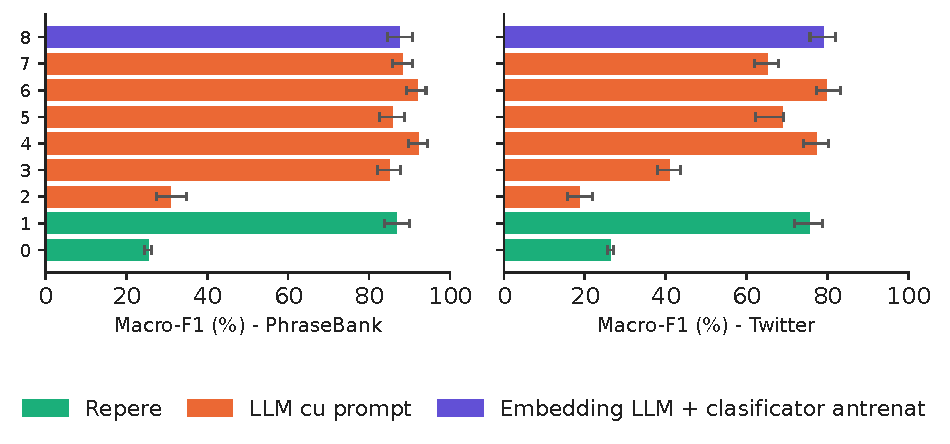
\includegraphics[width=\textwidth,height=0.442\textheight,keepaspectratio]{charts/ro/prompt_results.pdf}\end{center}\vspace{-3mm}
\chartsource{Sursa: Financial PhraseBank (Malo et al., 2014) și Twitter financial news (zeroshot). Date: seturi de test: 678 de propoziții (acord 100\,\%) și 900 de tweet-uri; intervale bootstrap de 95\,\%.}
\vspace{0.5mm}
\begin{itemize}\setlength{\itemsep}{0pt}
  \item Cel mai bun pe PhraseBank: zero-shot 3B (92{,}2\,\%)
    \begin{itemize}\setlength{\itemsep}{0pt}
      \item Pe Twitter: few-shot 3B (79{,}8\,\%)
      \item Zero-shot 3B: 92{,}2\,\% și 77{,}4\,\%.
    \end{itemize}
\end{itemize}
\par\vfill\noindent{\scriptsize\color{FooterGray}}\hfill\qlink{NN\_L12\_prompt\_results}{Quantlets/L12/NN_L12_prompt_results}\par\vspace{0.5mm}
\end{frame}

\begin{frame}{Acuratețea și macro-F1, cu intervale bootstrap de 95\,\%}
\small
{\scriptsize\renewcommand{\arraystretch}{1.05}\setlength{\tabcolsep}{4pt}
\begin{tabular}{@{}lrrlrrl@{}}\toprule
Metoda & Acur. & F1 & Int.\ 95\,\% & Acur. & F1 & Int.\ 95\,\% \\ \midrule
 & \multicolumn{3}{c}{PhraseBank} & \multicolumn{3}{c}{Twitter} \\
clasa majoritară & 61{,}4 & \cellcolor{Crimson!55}25{,}4 & [24{,}4; 26{,}3] & 65{,}6 & \cellcolor{Crimson!55}26{,}4 & [25{,}7; 27{,}1] \\
TF-IDF + logistică & 90{,}3 & \cellcolor{Forest!46}86{,}9 & [83{,}8; 90{,}0] & 81{,}4 & \cellcolor{Forest!46}75{,}5 & [71{,}9; 78{,}7] \\
zero-shot 0,5B & 62{,}8 & \cellcolor{Crimson!53}31{,}0 & [27{,}5; 34{,}8] & 23{,}1 & \cellcolor{Crimson!55}18{,}7 & [15{,}7; 21{,}9] \\
zero-shot 1,5B & 85{,}3 & \cellcolor{Forest!42}85{,}1 & [82{,}2; 87{,}9] & 37{,}8 & \cellcolor{Crimson!31}40{,}9 & [37{,}9; 43{,}7] \\
zero-shot 3B & 93{,}1 & \cellcolor{Forest!55}92{,}2 & [89{,}8; 94{,}4] & 81{,}2 & \cellcolor{Forest!50}77{,}4 & [74{,}2; 80{,}3] \\
few-shot 1,5B & 87{,}8 & \cellcolor{Forest!44}85{,}9 & [82{,}5; 88{,}7] & 73{,}7 & \cellcolor{Forest!31}68{,}8 & [62{,}3; 69{,}1] \\
few-shot 3B & 93{,}4 & \cellcolor{Forest!55}92{,}1 & [89{,}2; 94{,}1] & 84{,}3 & \cellcolor{Forest!55}79{,}8 & [77{,}2; 83{,}2] \\
chain-of-thought 3B & 88{,}5 & \cellcolor{Forest!48}88{,}4 & [85{,}7; 90{,}7] & 64{,}7 & \cellcolor{Forest!23}65{,}1 & [62{,}0; 68{,}0] \\
embedding 1,5B + logistică & 91{,}3 & \cellcolor{Forest!47}87{,}5 & [84{,}5; 90{,}7] & 83{,}0 & \cellcolor{Forest!53}79{,}0 & [75{,}7; 82{,}0] \\
\bottomrule\end{tabular}}
\par\vspace{0.5mm}{\scriptsize \begin{itemize}\setlength{\itemsep}{0pt}
  \item Macro-F1 = media celor trei scoruri F1 pe clase, astfel încît clasa mică negativă contează cît cea neutră; intervalele provin din 1.000 de reeșantionări bootstrap ale setului de test; few-shot = media a 3 rulări.
  \item Int. = intervalul bootstrap de 95\,\% al macro-F1.
\end{itemize}}
\par\vfill\noindent{\scriptsize\color{FooterGray}(calcul propriu)}\hfill\tryit{notebook \S3}\par\vspace{0.5mm}
\end{frame}

\begin{frame}{Cîteva exemple ajută modelul mic; mai multe exemple nu mai ajută}
\small
\intuition{învățarea în context: exemplele schimbă răspunsul fără să modifice nicio pondere.}
\vspace{-1mm}\[ \hat c=\argmax_c\,p_{\btheta}\big(c\mid (x_1,c_1),\dots,(x_k,c_k),x\big) \]\vspace{-2mm}
\begin{center}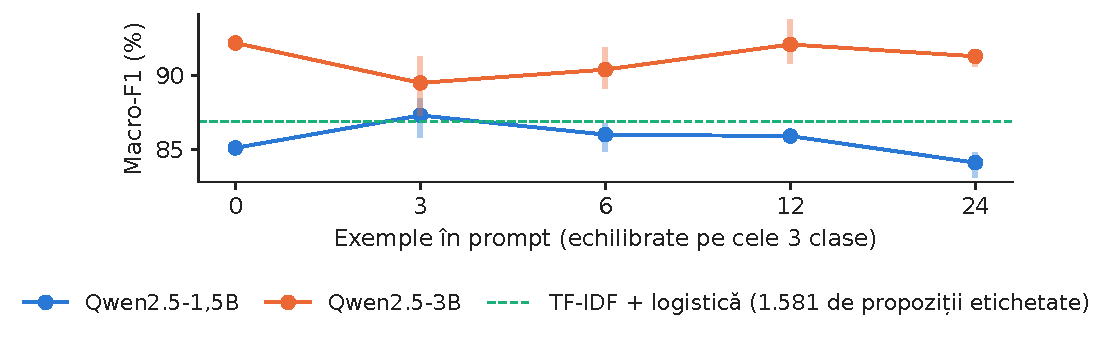
\includegraphics[width=\textwidth,height=0.421\textheight,keepaspectratio]{charts/ro/fewshot_curve.pdf}\end{center}\vspace{-3mm}
\chartsource{Sursa: Financial PhraseBank (Malo et al., 2014). Date: setul de test de 678 de propoziții; barele = intervalul pe 3 valori ale generatorului aleator.}
\vspace{0.5mm}
\begin{itemize}\setlength{\itemsep}{0pt}
  \item 1,5B: 85{,}1\,\% fără exemple, 84{,}1\,\% cu 24
    \begin{itemize}\setlength{\itemsep}{0pt}
      \item 3B: 92{,}2\,\% și 91{,}3\,\%
      \item Cu 12 exemple, rulările mută 3B între 91{,}0 și 93{,}6\,\%.
    \end{itemize}
\end{itemize}
\par\vfill\noindent{\scriptsize\color{FooterGray}}\hfill\qlink{NN\_L12\_fewshot\_curve}{Quantlets/L12/NN_L12_fewshot_curve}\par\vspace{0.5mm}
\end{frame}

\begin{frame}{Reformularea instrucțiunii schimbă scorul: sensibilitatea la prompt}
\small
\intuition{cinci instrucțiuni cu același sens, același model și aceleași date: diferențele sînt o sursă de risc de model.}
\begin{center}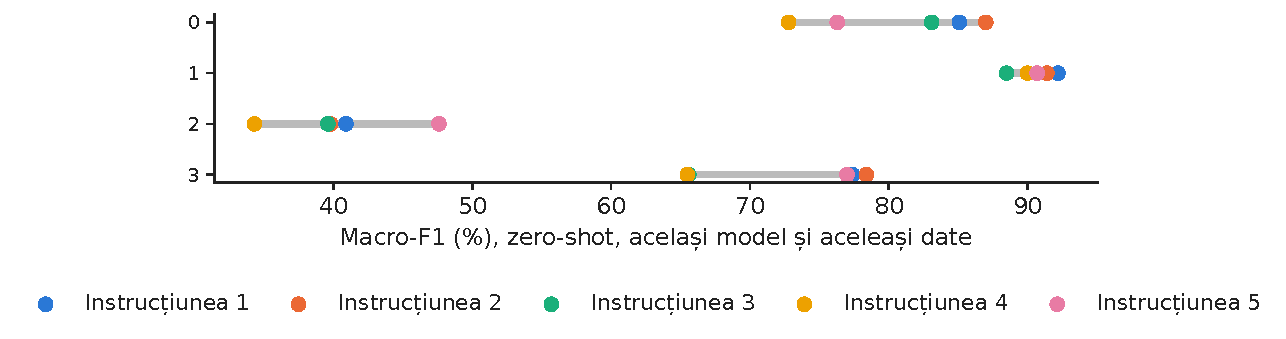
\includegraphics[width=\textwidth,height=0.353\textheight,keepaspectratio]{charts/ro/prompt_sensitivity.pdf}\end{center}\vspace{-3mm}
\chartsource{Sursa: Financial PhraseBank și Twitter financial news. Date: seturile de test de mai sus; cinci reformulări ale instrucțiunii.}
\vspace{0.5mm}
\begin{itemize}\setlength{\itemsep}{0pt}
  \item Amplitudinea macro-F1 pe cele cinci formulări: PhraseBank 3B 3{,}6 puncte, Twitter 3B 12{,}9 puncte, Twitter 1,5B 13{,}3 puncte.
\end{itemize}
\par\vfill\manager{alegeți promptul pe un set de validare și fixați-l, ca pe orice hiperparametru
    \begin{itemize}\setlength{\itemsep}{0pt}
      \item Niciodată pe setul de test.
    \end{itemize}}\par\vspace{0.5mm}
\par\vfill\noindent{\scriptsize\color{FooterGray}}\hfill\qlink{NN\_L12\_prompt\_sensitivity}{Quantlets/L12/NN_L12_prompt_sensitivity}\par\vspace{0.5mm}
\end{frame}

\begin{frame}{Chain-of-thought: modelul își scrie raționamentul înainte de răspuns}
\footnotesize
\intuition{tokenii de raționament generați devin context suplimentar pentru eticheta finală.}
\begin{columns}[T,onlytextwidth]
\begin{column}{0.53\textwidth}
\[ p(c\mid x)=\sum_{r}p(r\mid x)\,p(c\mid x,r)\ \approx\ p(c\mid x,\hat r) \]{\footnotesize\begin{itemize}\setlength{\itemsep}{0pt}
  \item \textbf{\txtwhere}
    \begin{itemize}\setlength{\itemsep}{0pt}
      \item $r$ = textul raționamentului, $\hat r$ = cel lacom (cel mult două propoziții, în medie 35{,}9 cuvinte)
      \item Eticheta se extrage din „Label: \ldots”
      \item Extragerea reușește pentru 100{,}0\,\% din răspunsurile PhraseBank.
    \end{itemize}
\end{itemize}\par}
\end{column}
\begin{column}{0.44\textwidth}
\begin{itemize}\setlength{\itemsep}{2pt}
  \item \textbf{Macro-F1}: PhraseBank 88{,}4\,\% (zero-shot 3B 92{,}2\,\%)
    \begin{itemize}\setlength{\itemsep}{0pt}
      \item Twitter 65{,}1\,\% (77{,}4\,\%).
    \end{itemize}
  \item \textbf{Costul}: 389 ms pe propoziție, față de 48{,}5 ms pentru zero-shot.
\end{itemize}
\end{column}
\end{columns}
\par\vfill\manager{chain-of-thought ajută la raționamente în mai mulți pași
    \begin{itemize}\setlength{\itemsep}{0pt}
      \item Pentru etichete de un cuvînt pe texte scurte, testați înainte să plătiți pentru el.
    \end{itemize}}\par\vspace{0.5mm}
\par\vfill\noindent{\scriptsize\color{FooterGray}(Wei et al., 2022)}\hfill\tryit{notebook \S5}\par\vspace{0.5mm}
\end{frame}

\begin{frame}{Ce a scris modelul: un răspuns chain-of-thought}
\small
\begin{itemize}\setlength{\itemsep}{4pt}
  \item \textbf{Intrare} (setul de test PhraseBank)
    \begin{itemize}\setlength{\itemsep}{0pt}
      \item ``CapMan said the deal 's effect on its cash flow for 2009 totals EUR3 .4 m , but the transaction would not affect its financial results for 2009 as it was executed at fair value .''
    \end{itemize}
  \item \textbf{Ieșirea} modelului Qwen2.5-3B-Instruct, temperatura 0
    \begin{itemize}\setlength{\itemsep}{0pt}
      \item ``Reasoning: The sentence indicates that the deal has a positive impact on CapMan's cash flow, which is generally seen as beneficial for investors. However, it also clarifies that the transaction does not affect their financial results, suggesting no immediate change to profitability. Given these points, the overall sentiment leans positive as it highlights a direct benefit. Label: positive''
    \end{itemize}
  \item \textbf{Cum se citește}
    \begin{itemize}\setlength{\itemsep}{0pt}
      \item Raționamentul este o poveste plauzibilă, nu o urmă fidelă a calculului
      \item Verificați eticheta pe date, nu explicația pe intuiție
    \end{itemize}
\end{itemize}
\par\vfill\noindent{\scriptsize\color{FooterGray}(calcul propriu)}\par\vspace{0.5mm}
\end{frame}

\begin{frame}{Sînt calibrate probabilitățile etichetelor? Fiabilitatea pe date reale}
\small
\intuition{o probabilitate de 0,9 trebuie să fie corectă de nouă ori din zece; punctele sub diagonală înseamnă încredere excesivă.}
\vspace{-1mm}\[ \mathrm{ECE}=\sum_{b=1}^{B}\frac{|S_b|}{n}\,\big|\mathrm{acc}(S_b)-\mathrm{conf}(S_b)\big| \]\vspace{-2mm}
\begin{center}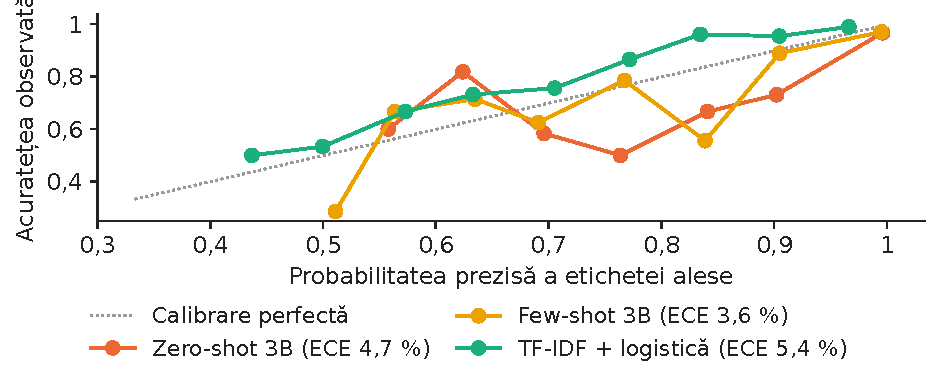
\includegraphics[width=\textwidth,height=0.308\textheight,keepaspectratio]{charts/ro/calibration.pdf}\end{center}\vspace{-3mm}
\chartsource{Sursa: Financial PhraseBank (Malo et al., 2014). Date: setul de test de 678 de propoziții, 10 intervale.}
\vspace{0.5mm}
\begin{itemize}\setlength{\itemsep}{0pt}
  \item Eroarea de calibrare așteptată (ECE): zero-shot 3B 4{,}7\,\%, few-shot 3B 3{,}6\,\%, TF-IDF + logistică 5{,}4\,\%.
\end{itemize}
\par\vfill\manager{recalibrați pe un set de validare (scalarea temperaturii) înainte de a folosi probabilitățile LLM ca scoruri de risc.}\par\vspace{0.5mm}
\par\vfill\noindent{\scriptsize\color{FooterGray}(Guo et al., 2017)}\hfill\qlink{NN\_L12\_calibration}{Quantlets/L12/NN_L12_calibration}\par\vspace{0.5mm}
\end{frame}

\begin{frame}{Acuratețea în funcție de gradul de acord al adnotatorilor}
\small
\intuition{propozițiile care îi împart pe adnotatori sînt cu adevărat ambigue; niciun model nu atinge pe ele acuratețea din cazurile unanime.}
\begin{center}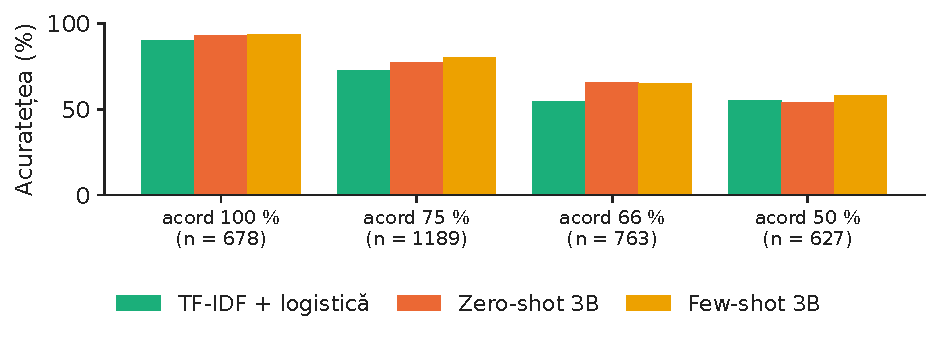
\includegraphics[width=\textwidth,height=0.365\textheight,keepaspectratio]{charts/ro/agreement.pdf}\end{center}\vspace{-3mm}
\chartsource{Sursa: Financial PhraseBank (Malo et al., 2014). Date: propoziții nefolosite nici la antrenare, nici ca exemple.}
\vspace{0.5mm}
\begin{itemize}\setlength{\itemsep}{0pt}
  \item Zero-shot 3B: 93{,}1\,\% la acord de 100\,\%, 53{,}7\,\% la 50\,\%
    \begin{itemize}\setlength{\itemsep}{0pt}
      \item TF-IDF: 90{,}3\,\% și 54{,}9\,\%.
    \end{itemize}
\end{itemize}
\par\vfill\manager{raportați calitatea etichetelor din setul de test
    \begin{itemize}\setlength{\itemsep}{0pt}
      \item Un model nu poate fi mai sigur decît oamenii care l-au etichetat.
    \end{itemize}}\par\vspace{0.5mm}
\par\vfill\noindent{\scriptsize\color{FooterGray}}\hfill\qlink{NN\_L12\_agreement}{Quantlets/L12/NN_L12_agreement}\par\vspace{0.5mm}
\end{frame}

\begin{frame}{Unde greșește cel mai bun prompt: matricea de confuzie}
\small
\begin{columns}[T,onlytextwidth]
\begin{column}{0.5\textwidth}
{\footnotesize\renewcommand{\arraystretch}{1.05}\setlength{\tabcolsep}{4pt}
\begin{tabular}{@{}lrrr@{}}\toprule
Real \textbackslash{} prezis & pozitiv & negativ & neutru \\ \midrule
pozitiv & \cellcolor{MainBlue!24}156 & 2 & \cellcolor{MainBlue!2}13 \\
negativ & 1 & \cellcolor{MainBlue!13}82 & \cellcolor{MainBlue!1}8 \\
neutru & \cellcolor{MainBlue!3}20 & 3 & \cellcolor{MainBlue!60}\textcolor{white}{393} \\
\bottomrule\end{tabular}}
\end{column}
\begin{column}{0.47\textwidth}
\begin{itemize}\setlength{\itemsep}{4pt}
  \item \textbf{Modelul}: zero-shot 3B, setul de test PhraseBank.
  \item \textbf{Neutru citit ca pozitiv}: 20 propoziții
    \begin{itemize}\setlength{\itemsep}{0pt}
      \item \textbf{pozitiv citit ca neutru}: 13.
    \end{itemize}
  \item \textbf{Negativ și pozitiv} se confundă rar: 1 + 2.
\end{itemize}
\end{column}
\end{columns}
\par\vspace{0.5mm}{\scriptsize \begin{itemize}\setlength{\itemsep}{0pt}
  \item Erorile stau la granița cu neutrul: „profitul a crescut, dar mai puțin decît se aștepta” este cazul dificil, nu știrile bune față de cele rele.
\end{itemize}}
\par\vfill\noindent{\scriptsize\color{FooterGray}(calcul propriu)}\hfill\tryit{notebook \S6}\par\vspace{0.5mm}
\end{frame}

\begin{frame}{Costul față de precizie: milisecunde pe propoziție, pe un laptop}
\small
\intuition{cel mai ieftin model este de mii de ori mai rapid decît cel mai lent; diferența de precizie este mică.}
\begin{center}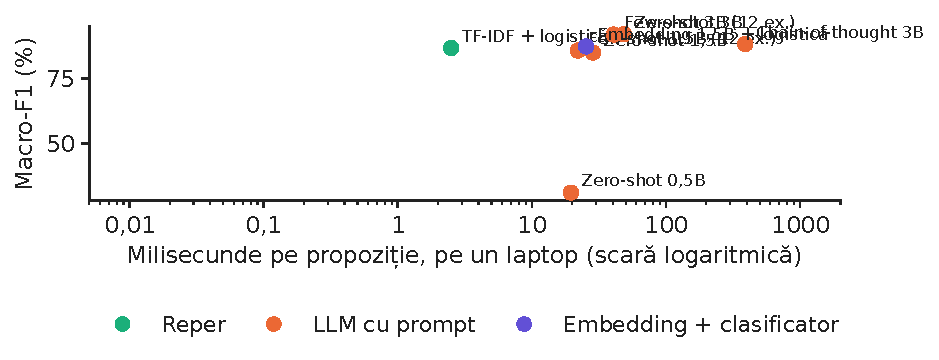
\includegraphics[width=\textwidth,height=0.238\textheight,keepaspectratio]{charts/ro/cost_accuracy.pdf}\end{center}\vspace{-3mm}
\chartsource{Sursa: Financial PhraseBank (Malo et al., 2014). Date: setul de test de 678 de propoziții; timp măsurat pe procesorul grafic al unui laptop.}
\vspace{0.5mm}
\begin{itemize}\setlength{\itemsep}{0pt}
  \item TF-IDF: 2{,}50 ms pe propoziție
    \begin{itemize}\setlength{\itemsep}{0pt}
      \item Zero-shot 3B: 48{,}5 ms
      \item Chain-of-thought 3B: 389 ms.
    \end{itemize}
\end{itemize}
\par\vfill\manager{dacă aveți etichete, antrenați un model mic
    \begin{itemize}\setlength{\itemsep}{0pt}
      \item Fără etichete, folosiți un prompt
      \item Pentru milioane de documente, costul decide.
    \end{itemize}}\par\vspace{0.5mm}
\par\vfill\noindent{\scriptsize\color{FooterGray}}\hfill\qlink{NN\_L12\_cost\_accuracy}{Quantlets/L12/NN_L12_cost_accuracy}\par\vspace{0.5mm}
\end{frame}

\begin{frame}{Embedding LLM plus un clasificator mic: cea mai ieftină formă de ajustare fină}
\footnotesize
\intuition{fixăm modelul de limbaj, facem media ultimelor stări ascunse și estimăm deasupra o regresie logistică.}
\begin{columns}[T,onlytextwidth]
\begin{column}{0.53\textwidth}
\[ \mathbf e(x)=\frac{1}{|x|}\sum_{t=1}^{|x|}\mathbf h^{(L)}_t,\qquad \hat p(c\mid x)=\softmax\big(\mathbf W\mathbf e(x)+\mathbf b\big)_c \]{\footnotesize\begin{itemize}\setlength{\itemsep}{0pt}
  \item \textbf{\txtwhere}
    \begin{itemize}\setlength{\itemsep}{0pt}
      \item $\mathbf h^{(L)}_t\in\R^{1536}$ = ultima stare ascunsă a Qwen2.5-1.5B
      \item $\mathbf W$ estimat cu penalizare L2 aleasă prin validare încrucișată în 5 pași.
    \end{itemize}
\end{itemize}\par}
\end{column}
\begin{column}{0.44\textwidth}
\begin{itemize}\setlength{\itemsep}{2pt}
  \item \textbf{Macro-F1}: PhraseBank 87{,}5\,\%, Twitter 79{,}0\,\%.
  \item \textbf{Folosește etichetele} ca TF-IDF, dar cu cunoștințele lingvistice ale LLM.
\end{itemize}
\end{column}
\end{columns}
\par\vfill\manager{înainte de o ajustare fină completă, încercați un clasificator pe embedding: cîteva minute pe laptop, fără gradient prin LLM.}\par\vspace{0.5mm}
\par\vfill\noindent{\scriptsize\color{FooterGray}}\hfill\tryit{notebook \S6}\par\vspace{0.5mm}
\end{frame}


\section{Generare augmentată prin regăsire pe discursurile BCE}

\begin{frame}{RAG: regăsim documentele potrivite, apoi modelul răspunde pe baza lor}
\small
\begin{center}\begin{tikzpicture}\node[draw, rounded corners, fill=MainBlue!12, text width=2.55cm, align=center, minimum height=1.05cm, font=\scriptsize] (n0) at (0.0,0) {\textbf{Întrebare}};\node[draw, rounded corners, fill=Ser3!12, text width=2.55cm, align=center, minimum height=1.05cm, font=\scriptsize] (n1) at (3.05,0) {\textbf{Regăsire}\\BM25 + dense\\primele $k$ fragmente};\node[draw, rounded corners, fill=Ser2!12, text width=2.55cm, align=center, minimum height=1.05cm, font=\scriptsize] (n2) at (6.1,0) {\textbf{Prompt}\\documente + întrebare};\node[draw, rounded corners, fill=Ser7!12, text width=2.55cm, align=center, minimum height=1.05cm, font=\scriptsize] (n3) at (9.149999999999999,0) {\textbf{Răspunsul LLM}\\cu surse};\draw[-{Stealth}, thick] (n0.east) -- (n1.west);\draw[-{Stealth}, thick] (n1.east) -- (n2.west);\draw[-{Stealth}, thick] (n2.east) -- (n3.west);\end{tikzpicture}\end{center}\vspace{-2mm}\[ p(y\mid q)\approx\sum_{z\in\mathrm{top}_k(q)}p_\eta(z\mid q)\,p_{\btheta}(y\mid q,z) \]\begin{itemize}\setlength{\itemsep}{2pt}
  \item \textbf{Generarea augmentată prin regăsire (RAG)}: $z$ = fragmentul regăsit, $p_\eta$ = modulul de regăsire, $p_{\btheta}$ = generatorul.
  \item \textbf{Corpusul nostru}: 400 de discursuri BCE, 8\,400 de fragmente de 200 de cuvinte (suprapunere 50).
\end{itemize}
\par\vfill\noindent{\scriptsize\color{FooterGray}(Lewis et al., 2020)}\par\vspace{0.5mm}
\end{frame}

\begin{frame}{Trei metode de regăsire: cuvinte comune, termeni ponderați, embedding}
\footnotesize
\intuition{metodele lexicale potrivesc cuvinte, cele dense sensul, iar metoda hibridă le combină; interogarea este titlul unui discurs.}
\begin{columns}[T,onlytextwidth]
\begin{column}{0.64\textwidth}
\[ \mathrm{BM25}(q,z)=\sum_{w\in q}\mathrm{idf}(w)\frac{f(w,z)(k_1+1)}{f(w,z)+k_1\big(1-b+b\frac{|z|}{\overline{|z|}}\big)} \]\[ s_{\text{dense}}=\cos\big(\mathbf e(q),\mathbf e(z)\big),\quad s_{\text{RRF}}(z)=\sum_{m}\frac{1}{60+\mathrm{rank}_m(z)} \]{\footnotesize\begin{itemize}\setlength{\itemsep}{0pt}
  \item \textbf{\txtwhere}
    \begin{itemize}\setlength{\itemsep}{0pt}
      \item $f(w,z)$ = aparițiile cuvîntului $w$ în fragmentul $z$
      \item $k_1=1{,}5$, $b=0{,}75$
      \item Best Matching 25 (BM25)
      \item $\mathbf e$ = embedding bge-small
      \item RRF = fuziunea rangurilor.
    \end{itemize}
\end{itemize}\par}
\end{column}
\begin{column}{0.33\textwidth}
\begin{itemize}\setlength{\itemsep}{2pt}
  \item \textbf{Rangul reciproc mediu (MRR)}: BM25 0{,}515, dense 0{,}567, hibrid 0{,}622.
\end{itemize}
\end{column}
\end{columns}
\par\vfill\manager{răspunsul nu poate fi mai bun decît ce s-a regăsit: evaluați întîi separat modulul de regăsire.}\par\vspace{0.5mm}
\par\vfill\noindent{\scriptsize\color{FooterGray}(Robertson \& Zaragoza, 2009; Xiao et al., 2023)}\hfill\tryit{notebook \S7}\par\vspace{0.5mm}
\end{frame}

\begin{frame}{Găsirea discursului corect după titlu}
\small
\intuition{recall@k = ponderea celor 400 de titluri pentru care discursul se află printre primele $k$ rezultate.}
\begin{center}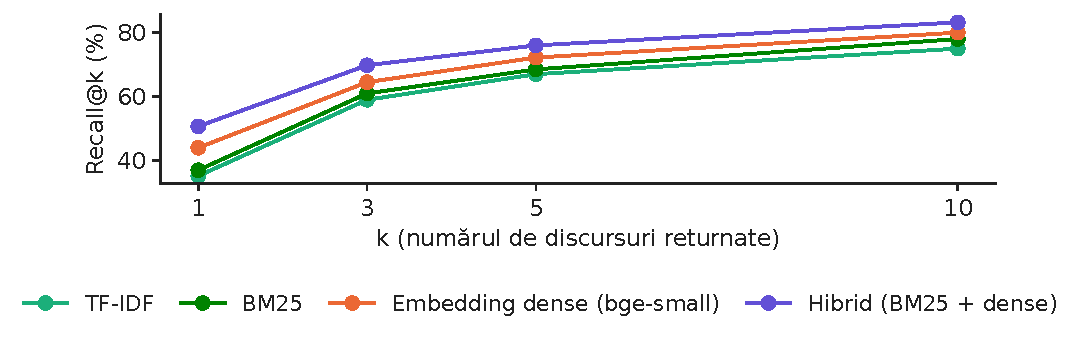
\includegraphics[width=\textwidth,height=0.500\textheight,keepaspectratio]{charts/ro/rag_recall.pdf}\end{center}\vspace{-3mm}
\chartsource{Sursa: Banca Centrală Europeană, setul de discursuri. Date: 400 de discursuri, 8400 de fragmente; interogarea = titlul discursului.}
\vspace{0.5mm}
\begin{itemize}\setlength{\itemsep}{0pt}
  \item Recall@1: TF-IDF 35{,}2\,\%, BM25 37{,}0\,\%, dense 44{,}0\,\%, hibrid 50{,}7\,\%
    \begin{itemize}\setlength{\itemsep}{0pt}
      \item Recall@10 hibrid 83{,}2\,\%.
    \end{itemize}
\end{itemize}
\par\vfill\noindent{\scriptsize\color{FooterGray}}\hfill\qlink{NN\_L12\_rag\_recall}{Quantlets/L12/NN_L12_rag_recall}\par\vspace{0.5mm}
\end{frame}

\begin{frame}{Răspunsurile cu și fără documente regăsite}
\small
\intuition{întrebarea: ce membru al conducerii a ținut discursul cu acest titlu? 160 de discursuri din 15 ianuarie 2025, ulterioare datelor de antrenare ale modelului.}
\begin{center}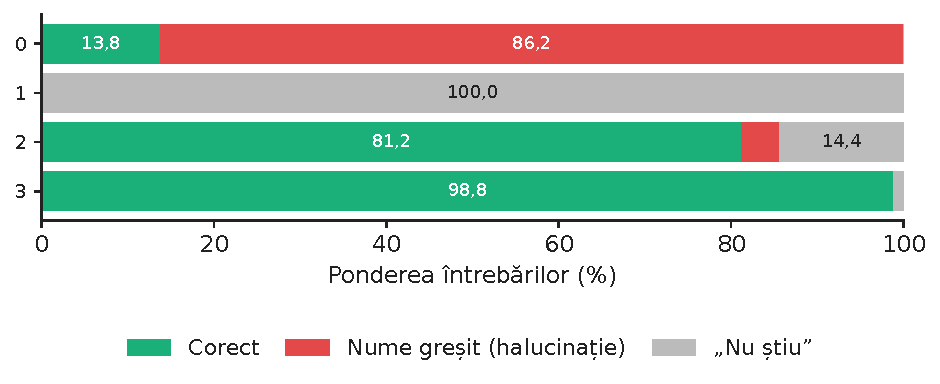
\includegraphics[width=\textwidth,height=0.348\textheight,keepaspectratio]{charts/ro/rag_qa.pdf}\end{center}\vspace{-3mm}
\chartsource{Sursa: Banca Centrală Europeană, setul de discursuri. Date: 160 de discursuri cu un singur vorbitor, 15 ianuarie 2025 - 30 octombrie 2026; modelul Qwen2.5-3B-Instruct.}
\vspace{0.5mm}
\begin{itemize}\setlength{\itemsep}{0pt}
  \item Răspuns obligatoriu fără documente: 86{,}2\,\% nume greșite, Philip Lane de 137 de ori
    \begin{itemize}\setlength{\itemsep}{0pt}
      \item RAG 81{,}2\,\% corecte, oracol 98{,}8\,\%
      \item Doar vorbitorul cel mai frecvent: 35{,}6\,\%.
    \end{itemize}
\end{itemize}
\par\vfill\manager{un nume greșit spus cu siguranță este eșecul costisitor: cereți surse în fiecare răspuns și verificați-le.}\par\vspace{0.5mm}
\par\vfill\noindent{\scriptsize\color{FooterGray}}\hfill\qlink{NN\_L12\_rag\_qa}{Quantlets/L12/NN_L12_rag_qa}\par\vspace{0.5mm}
\end{frame}

\begin{frame}{Proiectarea unui sistem RAG pentru o bancă: deciziile care contează}
\small
\begin{itemize}\setlength{\itemsep}{3pt}
  \item \textbf{Fragmentarea}
    \begin{itemize}\setlength{\itemsep}{0pt}
      \item Aici 200 de cuvinte cu suprapunere de 50; tabelele și notele de subsol au nevoie de reguli proprii
    \end{itemize}
  \item \textbf{Metadatele}
    \begin{itemize}\setlength{\itemsep}{0pt}
      \item Vorbitorul, data și titlul însoțesc fiecare fragment; răspunsul le citează
    \end{itemize}
  \item \textbf{Regăsirea}
    \begin{itemize}\setlength{\itemsep}{0pt}
      \item Hibrid BM25 + dense: recall@3 = 73{,}1\,\% pe discursurile folosite la întrebări
    \end{itemize}
  \item \textbf{Abținerea}
    \begin{itemize}\setlength{\itemsep}{0pt}
      \item Permiteți „nu știu”: fără documente, modelul se abține atunci la 100{,}0\,\% din întrebări
    \end{itemize}
  \item \textbf{Evaluarea}
    \begin{itemize}\setlength{\itemsep}{0pt}
      \item Un set fix de întrebări cu răspunsuri cunoscute, rulat din nou după fiecare modificare
    \end{itemize}
\end{itemize}
\end{frame}


\section{Modelele de limbaj ca modele de risc: LLM-VaR}

\begin{frame}{LLM-VaR: istoricul randamentelor în prompt, o cuantilă în răspuns}
\footnotesize
\intuition{fără estimare și fără ajustare fină: modelul citește 250 de randamente și scrie valoarea expusă la risc (VaR).}
\begin{columns}[T,onlytextwidth]
\begin{column}{0.53\textwidth}
\[ \widehat{\mathrm{VaR}}^{\alpha}_{t+1}=\mathrm{LLM}\big(\mathrm{prompt}(r_{t-249},\dots,r_t;\alpha)\big) \]\[ \mathrm{LR}_{uc}=-2\ln\frac{(1-\alpha)^{n_0}\alpha^{n_1}}{(1-\hat\pi)^{n_0}\hat\pi^{n_1}}\sim\chi^2_1 \]{\footnotesize\begin{itemize}\setlength{\itemsep}{0pt}
  \item \textbf{\txtwhere}
    \begin{itemize}\setlength{\itemsep}{0pt}
      \item $r_t$ = randamentul logaritmic zilnic al S\&P 500 (\%)
      \item $\alpha\in\{1\,\%,5\,\%\}$
      \item Temperatura 0
      \item $n_1$ = depășirile
      \item Testul raportului de verosimilitate (LR) Kupiec.
    \end{itemize}
\end{itemize}\par}
\end{column}
\begin{column}{0.44\textwidth}
\begin{itemize}\setlength{\itemsep}{2pt}
  \item \textbf{Replicarea noastră}: Qwen2.5-3B-Instruct, 459 de zile, din 2 ianuarie 2025 pînă la 30 octombrie 2026.
  \item \textbf{Repere}: simularea istorică (HS), 250 de zile
    \begin{itemize}\setlength{\itemsep}{0pt}
      \item Heteroscedasticitate condiționată autoregresivă generalizată (GARCH), GARCH(1,1)-$t$.
    \end{itemize}
\end{itemize}
\end{column}
\end{columns}
\par\vfill\manager{un model deschis de 3B pe laptop este cel mai ieftin test al ideii
    \begin{itemize}\setlength{\itemsep}{0pt}
      \item Lucrarea a folosit modele comerciale mari.
    \end{itemize}}\par\vspace{0.5mm}
\par\vfill\noindent{\scriptsize\color{FooterGray}(Pele et al., 2026; Kupiec, 1995)}\hfill\tryit{notebook \S9}\par\vspace{0.5mm}
\end{frame}

\begin{frame}{LLM-VaR cu un model deschis de 3B pe S\&P 500}
\small
\intuition{VaR de 5\,\% a modelului de limbaj comparată cu GARCH; punctele roșii marchează zilele în care LLM-VaR a fost depășită.}
\begin{center}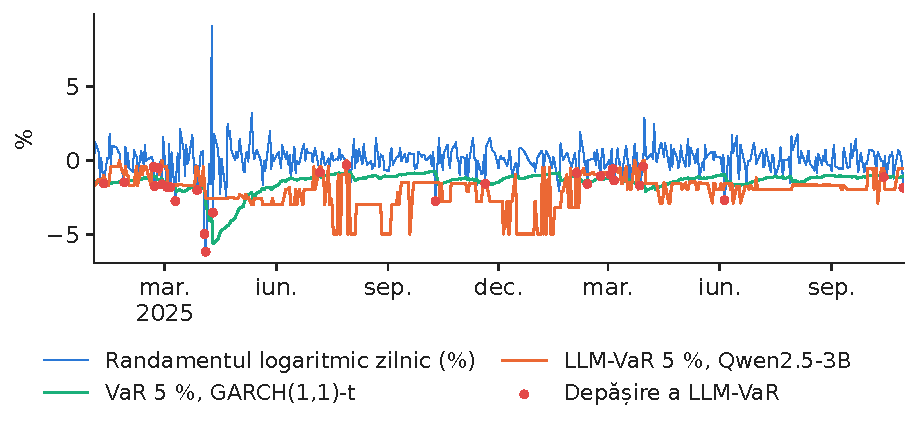
\includegraphics[width=\textwidth,height=0.468\textheight,keepaspectratio]{charts/ro/llm_var.pdf}\end{center}\vspace{-3mm}
\chartsource{Sursa: Yahoo Finance, cotații zilnice. Date: 2 ianuarie 2025 - 30 octombrie 2026, S\&P 500, zile de tranzacționare.}
\vspace{0.5mm}
\begin{itemize}\setlength{\itemsep}{0pt}
  \item 5\,\%: LLM 28 depășiri, GARCH 35, HS 23, așteptate 23{,}0.
  \item VaR medie de 5\,\%: LLM \ensuremath{-}1{,}99\,\%, GARCH \ensuremath{-}1{,}42\,\%
    \begin{itemize}\setlength{\itemsep}{0pt}
      \item Corelația lor 0{,}05: modelul mic acoperă riscul fiind prudent, nu urmărind volatilitatea.
    \end{itemize}
\end{itemize}
\par\vfill\noindent{\scriptsize\color{FooterGray}}\hfill\qlink{NN\_L12\_llm\_var}{Quantlets/L12/NN_L12_llm_var}\par\vspace{0.5mm}
\end{frame}

\begin{frame}{Testarea retrospectivă a LLM-VaR față de reperele clasice}
\small
{\footnotesize\renewcommand{\arraystretch}{1.05}\setlength{\tabcolsep}{4pt}
\begin{tabular}{@{}lrrrrrrr@{}}\toprule
Model & Dep.\ 1\,\% & Rata (\%) & $p_{uc}$ & Dep.\ 5\,\% & Rata (\%) & $p_{uc}$ & VaR 5\,\% medie \\ \midrule
LLM-VaR (Qwen2.5-3B) & 4 & 0{,}87 & \cellcolor{Forest!55}0{,}777 & 28 & 6{,}10 & \cellcolor{Forest!55}0{,}295 & \ensuremath{-}1{,}99 \\
HS (250 de zile) & 6 & 1{,}31 & \cellcolor{Forest!55}0{,}528 & 23 & 5{,}01 & \cellcolor{Forest!55}0{,}991 & \ensuremath{-}1{,}56 \\
GARCH(1,1)-$t$ & 9 & 1{,}96 & \cellcolor{Forest!19}0{,}067 & 35 & 7{,}63 & \cellcolor{Crimson!37}0{,}016 & \ensuremath{-}1{,}42 \\
\bottomrule\end{tabular}}
\par\vspace{0.5mm}{\scriptsize \begin{itemize}\setlength{\itemsep}{0pt}
  \item Depășiri așteptate: 4{,}6 la 1\,\% și 23{,}0 la 5\,\%; valoare $p$ verde: acoperirea nu este respinsă la 10\,\%.
  \item Răspunsuri citite ca număr: 100{,}0\,\% la 5\,\%, 100{,}0\,\% la 1\,\%; un răspuns ilizibil păstrează valoarea din ziua precedentă.
  \item Dimensiunea modelului contează: studiul publicat a evaluat modele mult mai mari; rezultatele de aici descriu doar un model de 3B.
\end{itemize}}
\par\vfill\noindent{\scriptsize\color{FooterGray}(calcul propriu; Pele et al., 2026)}\hfill\tryit{notebook \S9}\par\vspace{0.5mm}
\end{frame}


\section{Riscuri și guvernanță}

\begin{frame}{Șase riscuri ale LLM într-o instituție financiară și testul pentru fiecare}
\small
{\scriptsize\renewcommand{\arraystretch}{1.05}\setlength{\tabcolsep}{4pt}
\begin{tabular}{@{}p{0.2\textwidth}p{0.38\textwidth}p{0.36\textwidth}@{}}\toprule
Risc & Observat în acest curs & Control \\ \midrule
Halucinația & 86{,}2\,\% nume greșite fără documente & RAG cu surse; abținerea permisă \\
Scurgerea datelor & perplexitate mai mică pe discursurile vechi & testare pe texte ulterioare limitei datelor \\
Sensibilitatea la prompt & 12{,}9 puncte macro-F1 între formulări & selecție pe validare, fixare, versionare \\
Calibrarea & ECE 4{,}7\,\% zero-shot, 5{,}4\,\% TF-IDF & scalarea temperaturii, praguri stabilite pe validare \\
Costul și latența & 389 ms față de 2{,}50 ms pe propoziție & cel mai mic model care trece testul \\
Protecția datelor & documente ale clienților în prompturi & modele locale; obligațiile din Regulamentul Uniunii Europene (UE) privind inteligența artificială (AI) pentru utilizările cu risc ridicat, precum scoringul de credit \\
\bottomrule\end{tabular}}
\par\vspace{0.5mm}{\scriptsize \begin{itemize}\setlength{\itemsep}{0pt}
  \item Regulamentul (UE) 2024/1689 privind inteligența artificială.
\end{itemize}}
\end{frame}

\section*{Recapitulare}

\begin{frame}{Test 1: temperatura}
\small
\begin{itemize}
  \item Clasificați 10.000 de știri cu un LLM și obțineți etichete diferite la două rulări pentru aceeași știre
    \begin{itemize}\setlength{\itemsep}{0pt}
      \item Ce schimbați mai întîi?
    \end{itemize}
\end{itemize}
\vspace{2mm}
\begin{exampleblock}{R\u{a}spuns}
\begin{itemize}
  \item Setați temperatura la 0 (sau citiți probabilitățile etichetelor): eșantionarea la $T>0$ este aleatoare prin construcție.
\end{itemize}
\end{exampleblock}
\end{frame}

\begin{frame}{Test 2: evaluarea}
\small
\begin{itemize}
  \item Un furnizor raportează o acuratețe de 95\,\% a LLM-ului său pe Financial PhraseBank
    \begin{itemize}\setlength{\itemsep}{0pt}
      \item Ce două întrebări puneți?
    \end{itemize}
\end{itemize}
\vspace{2mm}
\begin{exampleblock}{R\u{a}spuns}
\begin{itemize}
  \item Pe ce subset de acord (cel unanim este cel mai ușor) și a fost PhraseBank în datele de antrenare (publicat în 2014, copiat pe scară largă)? Cereți și macro-F1: 61{,}4\,\% dintre propoziții sînt neutre.
\end{itemize}
\end{exampleblock}
\end{frame}

\begin{frame}{Test 3: RAG}
\small
\begin{itemize}
  \item Asistentul RAG răspunde greșit, deși documentul corect există în corpus
    \begin{itemize}\setlength{\itemsep}{0pt}
      \item Unde căutați mai întîi?
    \end{itemize}
\end{itemize}
\vspace{2mm}
\begin{exampleblock}{R\u{a}spuns}
\begin{itemize}
  \item La modulul de regăsire: verificați dacă documentul este printre primele $k$ (recall@k)
    \begin{itemize}\setlength{\itemsep}{0pt}
      \item Abia apoi la prompt și la model.
    \end{itemize}
\end{itemize}
\end{exampleblock}
\end{frame}

\begin{frame}{Recapitulare}
\small
\begin{itemize}\setlength{\itemsep}{4pt}
  \item Un LLM este un model al următorului token
    \begin{itemize}\setlength{\itemsep}{0pt}
      \item Perplexitatea, temperatura și tokenii sînt mărimile sale de bază.
    \end{itemize}
  \item Un prompt este un model: evaluați-l pe etichete separate, cu intervale, rulări repetate și reformulări.
  \item Cu etichete, modelele mici antrenate și embedding-urile LLM sînt greu de depășit
    \begin{itemize}\setlength{\itemsep}{0pt}
      \item Fără etichete, prompturile oferă un început solid.
    \end{itemize}
  \item RAG transformă răspunsurile inventate în răspunsuri cu surse
    \begin{itemize}\setlength{\itemsep}{0pt}
      \item Evaluați întîi modulul de regăsire.
    \end{itemize}
  \item Urmează: modelele fundație pentru serii de timp din energie și finanțe (cursul 13).
\end{itemize}
\end{frame}

\begin{frame}{Cercetările grupului nostru}
\footnotesize
\begin{itemize}\setlength{\itemsep}{4pt}
  \item \textbf{LLM-VaR și, pentru pierderea așteptată în coada distribuției (ES), LLM-ES}: LLM-uri generale estimează, fără reantrenare, ambele măsuri de risc dintr-un prompt structurat cu randamentele trecute
    \begin{itemize}\setlength{\itemsep}{0pt}
      \item Testate retrospectiv față de modelele clasice de risc (Pele, Bolovăneanu, Lin, Ren, Ginavar, Spilak, Andrei, Toma, Lessmann \& Härdle, 2026, Expert Systems with Applications).
    \end{itemize}
  \item \textbf{Prognoza acțiunilor cu LLM}: LLaMA 3.3 combină în prompt istoricul prețurilor cu sentimentul știrilor și depășește LLaMA 3.1 și un model autoregresiv integrat cu medie mobilă (Tak \& Pele, 2025, PICBE).
  \item \textbf{Narațiunile băncii centrale}: un indice de sentiment construit cu un model transformer din minutele Băncii Naționale a României îmbunătățește prognoza inflației (Amza, Bolovăneanu \& Pele, 2026, PICBE) --- același tip de text ca discursurile BCE din acest curs.
\end{itemize}
\par\vspace{0.5mm}{\scriptsize \begin{itemize}\setlength{\itemsep}{0pt}
  \item Rezultatele sînt preluate din rezumatele lucrărilor; cifrele de pe celelalte slide-uri provin din datele noastre.
\end{itemize}}
\par\vfill\noindent{\scriptsize\color{FooterGray}(Academia de Studii Economice din București, ASE; Academia Română, Institutul de Prognoză Economică, IPE)}\par\vspace{0.5mm}
\end{frame}

\begin{frame}{Vreți să aflați mai mult?}
\small
\begin{columns}[T,onlytextwidth]
\begin{column}{0.5\textwidth}
\begin{itemize}\setlength{\itemsep}{4pt}
  \item \textbf{Hugging Face}, curs despre LLM: \href{https://huggingface.co/learn/llm-course}{huggingface.co/learn/llm-course}.
  \item \textbf{Qwen2.5}, modele și raport: \href{https://huggingface.co/Qwen}{huggingface.co/Qwen}.
  \item \textbf{Ghid de formulare a prompturilor}: \href{https://www.promptingguide.ai}{promptingguide.ai}.
\end{itemize}
\end{column}
\begin{column}{0.47\textwidth}
\begin{itemize}\setlength{\itemsep}{4pt}
  \item \textbf{Setul de discursuri BCE}: \href{https://www.ecb.europa.eu/press/key/html/downloads.en.html}{ecb.europa.eu}.
  \item \textbf{Quantinar}: The Next Word Problem: \href{https://quantinar.com/course/100100/the-next-word-problem-full-course}{quantinar.com}.
  \item \textbf{Acest curs}: notebook, seminar și Quantlets --- \href{https://github.com/danpele/NEURAL_BIZ}{github.com/danpele/NEURAL\_BIZ}.
\end{itemize}
\end{column}
\end{columns}
\end{frame}

\begin{frame}{Bibliografie (1/2)}
\scriptsize
\begin{itemize}\setlength{\itemsep}{0pt}\scriptsize
\item Amza, A., Bolovăneanu, V.\ \& Pele, D.\,T.\ (2026). Inflation forecasting with monetary policy narratives: Evidence from an emerging economy. \textit{Proceedings of the International Conference on Business Excellence}, 20(1), 75--83. \href{https://doi.org/10.2478/picbe-2026-0012}{doi:10.2478/picbe-2026-0012}
\item Brown, T.\,B.\ et al.\ (2020). Language models are few-shot learners. \textit{Advances in Neural Information Processing Systems}, 33. \href{https://arxiv.org/abs/2005.14165}{arXiv:2005.14165}
\item Guo, C., Pleiss, G., Sun, Y.\ \& Weinberger, K.\,Q.\ (2017). On calibration of modern neural networks. \textit{Proceedings of the 34th International Conference on Machine Learning}, 1321--1330. \href{https://arxiv.org/abs/1706.04599}{arXiv:1706.04599}
\item Hoffmann, J.\ et al.\ (2022). Training compute-optimal large language models. \textit{Advances in Neural Information Processing Systems}, 35. \href{https://arxiv.org/abs/2203.15556}{arXiv:2203.15556}
\item Hu, E.\,J., Shen, Y., Wallis, P., Allen-Zhu, Z., Li, Y., Wang, S., Wang, L.\ \& Chen, W.\ (2022). LoRA: Low-rank adaptation of large language models. \textit{International Conference on Learning Representations}. \href{https://arxiv.org/abs/2106.09685}{arXiv:2106.09685}
\item Kaplan, J.\ et al.\ (2020). Scaling laws for neural language models. \href{https://arxiv.org/abs/2001.08361}{arXiv:2001.08361}
\item Kupiec, P.\,H.\ (1995). Techniques for verifying the accuracy of risk measurement models. \textit{The Journal of Derivatives}, 3(2), 73--84. \href{https://doi.org/10.3905/jod.1995.407942}{doi:10.3905/jod.1995.407942}
\item Lewis, P.\ et al.\ (2020). Retrieval-augmented generation for knowledge-intensive NLP tasks. \textit{Advances in Neural Information Processing Systems}, 33. \href{https://arxiv.org/abs/2005.11401}{arXiv:2005.11401}
\item Malo, P., Sinha, A., Korhonen, P., Wallenius, J.\ \& Takala, P.\ (2014). Good debt or bad debt: Detecting semantic orientations in economic texts. \textit{Journal of the Association for Information Science and Technology}, 65(4), 782--796. \href{https://doi.org/10.1002/asi.23062}{doi:10.1002/asi.23062}
\item Ouyang, L.\ et al.\ (2022). Training language models to follow instructions with human feedback. \textit{Advances in Neural Information Processing Systems}, 35. \href{https://arxiv.org/abs/2203.02155}{arXiv:2203.02155}
\end{itemize}
\end{frame}

\begin{frame}{Bibliografie (2/2)}
\scriptsize
\begin{itemize}\setlength{\itemsep}{0pt}\scriptsize
\item Pele, D.\,T., Bolovăneanu, V., Lin, M.-B., Ren, R., Ginavar, A.\,T., Spilak, B., Andrei, A.-V., Toma, F.-M., Lessmann, S.\ \& Härdle, W.\,K.\ (2026). In the beginning was the Word: LLM-VaR and LLM-ES. \textit{Expert Systems with Applications}, 295, 128676. \href{https://doi.org/10.1016/j.eswa.2025.128676}{doi:10.1016/j.eswa.2025.128676}
\item Qwen Team (2024). Qwen2.5 technical report. \href{https://arxiv.org/abs/2412.15115}{arXiv:2412.15115}
\item Rafailov, R., Sharma, A., Mitchell, E., Ermon, S., Manning, C.\,D.\ \& Finn, C.\ (2023). Direct preference optimization: Your language model is secretly a reward model. \textit{Advances in Neural Information Processing Systems}, 36. \href{https://arxiv.org/abs/2305.18290}{arXiv:2305.18290}
\item Robertson, S.\ \& Zaragoza, H.\ (2009). The probabilistic relevance framework: BM25 and beyond. \textit{Foundations and Trends in Information Retrieval}, 3(4), 333--389. \href{https://doi.org/10.1561/1500000019}{doi:10.1561/1500000019}
\item Sennrich, R., Haddow, B.\ \& Birch, A.\ (2016). Neural machine translation of rare words with subword units. \textit{Proceedings of the 54th Annual Meeting of the ACL}, 1715--1725. \href{https://doi.org/10.18653/v1/P16-1162}{doi:10.18653/v1/P16-1162}
\item Tak, R.\ \& Pele, D.\,T.\ (2025). LLM-driven stock prediction: Capturing market trends with LLaMA. \textit{Proceedings of the International Conference on Business Excellence}, 19(1), 529--540. \href{https://doi.org/10.2478/picbe-2025-0043}{doi:10.2478/picbe-2025-0043}
\item Wei, J.\ et al.\ (2022). Chain-of-thought prompting elicits reasoning in large language models. \textit{Advances in Neural Information Processing Systems}, 35. \href{https://arxiv.org/abs/2201.11903}{arXiv:2201.11903}
\item Xiao, S., Liu, Z., Zhang, P.\ \& Muennighoff, N.\ (2023). C-Pack: Packaged resources to advance general Chinese embedding (BAAI general embedding). \href{https://arxiv.org/abs/2309.07597}{arXiv:2309.07597}
\item Zhao, Z., Wallace, E., Feng, S., Klein, D.\ \& Singh, S.\ (2021). Calibrate before use: Improving few-shot performance of language models. \textit{Proceedings of the 38th International Conference on Machine Learning}, 12697--12706. \href{https://arxiv.org/abs/2102.09690}{arXiv:2102.09690}
\end{itemize}
\end{frame}

\appendix

\section*{Anexă}

\begin{frame}{Anexa A: promptul folosit pentru clasificarea zero-shot}
\small
\begin{itemize}\setlength{\itemsep}{4pt}
  \item \textbf{Sistem}
    \begin{itemize}\setlength{\itemsep}{0pt}
      \item ``You are a careful financial analyst.''
    \end{itemize}
  \item \textbf{Utilizator}
    \begin{itemize}\setlength{\itemsep}{0pt}
      \item ``Classify the sentiment of this sentence from financial news, from the point of view of an investor in the company. Answer with one word: positive, negative or neutral. Sentence: \ldots{} Answer:''
    \end{itemize}
  \item \textbf{Few-shot}
    \begin{itemize}\setlength{\itemsep}{0pt}
      \item La fel, cu perechi „Sentence: \ldots{} Answer: etichetă” înaintea intrării; exemple echilibrate pe clase și amestecate
    \end{itemize}
  \item \textbf{Chain-of-thought}
    \begin{itemize}\setlength{\itemsep}{0pt}
      \item ``\ldots{} First explain your reasoning in at most two short sentences, then give the final answer on a new line as `Label: <positive|negative|neutral>'.''
    \end{itemize}
\end{itemize}
\end{frame}

\begin{frame}{Anexa B: detalii de implementare}
\small
\begin{itemize}\setlength{\itemsep}{4pt}
  \item Modele în float16, pe procesorul grafic al laptopului (PyTorch)
    \begin{itemize}\setlength{\itemsep}{0pt}
      \item Biblioteca Hugging Face transformers
      \item Scikit-learn pentru TF-IDF, regresia logistică și bootstrap.
    \end{itemize}
  \item Valorile generatorului aleator: 20261108 pentru împărțiri și eșantioane
    \begin{itemize}\setlength{\itemsep}{0pt}
      \item Exemplele few-shot cu valorile 20261108, +1 și +2.
    \end{itemize}
  \item Întreaga analiză a durat 2{,}2 minute la ultima rulare (ieșirile modelelor stocate)
    \begin{itemize}\setlength{\itemsep}{0pt}
      \item Prima rulare, aproximativ 40 de minute.
    \end{itemize}
  \item Predicțiile pentru fiecare element sînt publicate împreună cu Quantlet-urile, astfel încît fiecare cifră poate fi recalculată fără placă grafică.
\end{itemize}
\end{frame}

\end{document}
